\documentclass[conference]{IEEEtran}
\IEEEoverridecommandlockouts
\usepackage{cite}
\usepackage{amsmath,amssymb,amsfonts}
\usepackage{algorithmic}
\usepackage{graphicx}
\usepackage{textcomp}
\usepackage{xcolor}
\usepackage{tabularx}
\usepackage{hyperref}
\def\BibTeX{{\rm B\kern-.05em{\sc i\kern-.025em b}\kern-.08em
    T\kern-.1667em\lower.7ex\hbox{E}\kern-.125emX}}
\begin{document}

\title{GPU-Accelerated Density Functional Theory Solver for Binary SALR Colloids (SALR3YUCUDA)}

\author{
\IEEEauthorblockN{Nazar Pasichnyk}
\IEEEauthorblockA{\textit{Faculty of Applied Sciences} \\
\textit{Ukrainian Catholic University}\\
Lviv, Ukraine \\
pasichnyk.pn@ucu.edu.ua}
\and
\IEEEauthorblockN{Roman Prokhorov}
\IEEEauthorblockA{\textit{Faculty of Applied Sciences} \\
\textit{Ukrainian Catholic University}\\
Lviv, Ukraine \\
prokhorov.pn@ucu.edu.ua}
\and
\IEEEauthorblockN{Taras Patsahan}
\IEEEauthorblockA{\textit{Yukhnovskii Institute for Condensed Matter Physics,} \\
\textit{NAS of Ukraine}\\
Lviv, Ukraine \\
tarpa@icmp.lviv.ua}
}

\maketitle

\begin{abstract}
We present a computational framework for solving mean-field density functional theory (DFT) equations for spatial density distributions in binary colloidal mixtures with competing short-range attraction and long-range repulsion (SALR) interactions. The SALR pair potential is represented by a three-Yukawa form. The solver implements the Picard iterative procedure for a two-component system under different boundary conditions. Our CPU implementation employs OpenMP parallelization, achieving significant speedup on multi-core processors. A CUDA implementation for GPUs was developed, delivering a multi-fold speedup over the CPU baseline. On the laptop benchmark, the GPU run was $5.15\times$ faster than a 20-thread OpenMP execution, and the cluster run reached $70.85\times$ speedup over a single-thread CPU baseline. We demonstrate the solver capabilities by computing equilibrium density profiles under periodic, two-wall, and four-wall boundary conditions. A Qt-based graphical user interface (GUI) was also built to facilitate parameter configuration, task execution, and result visualization.
\end{abstract}

%--------------------------
\section{Introduction}
%--------------------------
Colloidal systems are an important class of soft-matter systems widely used for studying fundamental phenomena such as phase transitions, self-assembly, and the behaviour of complex fluids~\cite{royall2018}. Particularly intriguing are colloidal systems in which the pair interactions are competing in nature, combining short-range attraction with long-range repulsion (SALR).
These interactions, sometimes referred to as ``mermaid'' potentials because of their attractive head and repulsive tail~\cite{royall2018}.  
Systems of particles with SALR interactions can undergo microphase separation, giving rise to rich phase behaviour and mesoscopic structures such as ordered clusters and periodic stripe patterns~\cite{liu2019}. Figure~\ref{fig:mermaid} illustrates a typical SALR potential profile, with the short-range attractive well (``head'') followed by a long-range repulsive barrier (``tail'').

\begin{figure}[htbp]
\centerline{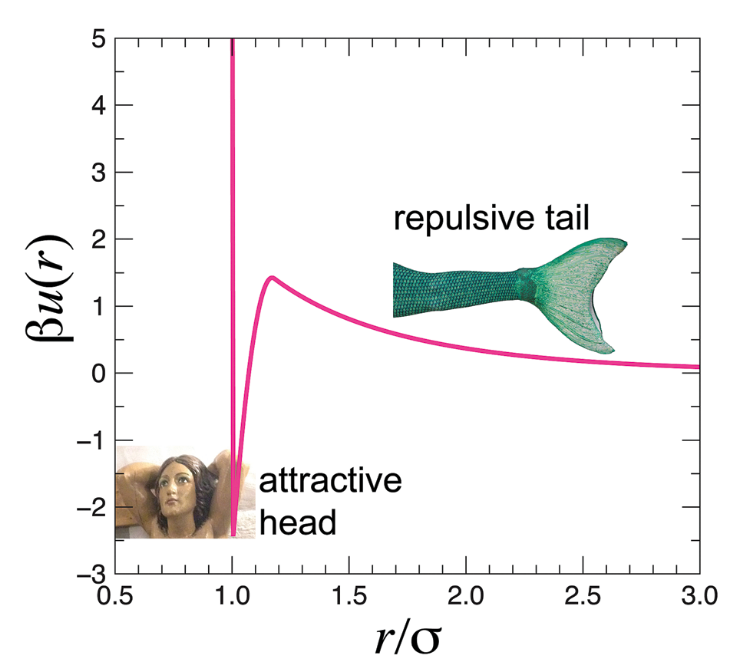
\includegraphics[width=0.85\columnwidth]{src/Mermaid_Chart.png}}
\caption{A ``mermaid'' (SALR) pair potential as a function of reduced separation $r/\sigma$. The attractive head promotes local condensation while the repulsive tail prevents bulk phase separation, driving the system toward microphase-separated morphologies such as clusters and stripes. Reproduced from~\cite{royall2018}.}
\label{fig:mermaid}
\end{figure}

Despite significant theoretical progress in predicting the behaviour of SALR systems, the experimental realization of the predicted mesophases in three-dimensional real space remains challenging. As Royall notes, ``no ordered phase in a system with competing interactions has ever been observed in 3d real space''~\cite{royall2018}. This gap between theory and experiment motivates the development of efficient computational tools that allow researchers to explore parameter space rapidly and identify conditions under which specific morphologies may emerge.

Theoretical descriptions of spatial density distributions in SALR systems are commonly based on density functional theory (DFT) within the mean-field approximation~\cite{hansen2013}. This approach leads to a system of nonlinear integral equations that must be solved iteratively. For a two-dimensional grid of $N_x \times N_y$ nodes, the computational cost per iteration scales as $O(N^2)$ due to the convolution required to compute interaction fields, making the problem computationally intensive.

In this work, we present SALR3YUCUDA, a computational solver for mean-field DFT equations describing spatial density distributions in binary mixtures of SALR particles. The project name reflects its key components: SALR (Short-range Attraction Long-range Repulsion), 3Y (three-Yukawa potential), and CUDA (GPU acceleration technology). We implemented an optimized pure C version with OpenMP parallelization for scalable execution on multi-core processors, accompanied by a highly parallelized CUDA framework for GPU-accelerated massive parameter computations. The solvers natively integrate with an SQLite-HDF5 database for session tracking and large spatial tensor storage, and feature multiple boundary conditions including periodic boundaries (PBC), two parallel walls (W2), and four-wall confinement (W4). Furthermore, a Qt-based graphical interface enables rich visual exploration without cumbersome command-line workflows.

\subsection{Motivation}

Binary colloidal mixtures with SALR interactions are of fundamental interest across soft matter, biophysics, and materials science. The interplay of competing attraction and repulsion gives rise to self-assembled mesophases - clusters, stripes, and lamellar structures - that serve as model systems for understanding protein aggregation, lipid membranes, and block-copolymer microphase separation~\cite{royall2018,liu2019}. Mapping the conditions under which each morphology appears requires systematic exploration of a high-dimensional parameter space (composition, temperature, interaction strengths and ranges), which is experimentally costly and time-consuming.

Particle-resolved computer simulations such as molecular dynamics (MD) and Monte Carlo (MC) provide the most detailed description of these systems, tracking every particle trajectory and configuration. However, their computational cost scales with the number of particles $N_p$: a single equilibration run for a system large enough to contain several stripe periods may require millions of MC sweeps or nanoseconds of MD trajectory, making large-scale parameter surveys impractical. Furthermore, finite-size effects are pronounced when the system box is not much larger than the characteristic pattern wavelength.

Density functional theory offers a complementary approach that avoids these limitations. Rather than evolving individual particle positions, DFT works directly with continuous density fields $\rho_i(\mathbf{r})$, reducing an $N_p$-body statistical mechanics problem to a deterministic nonlinear integral equation solved on an $N_x \times N_y$ grid. Key advantages include:

\begin{itemize}
    \item \textbf{Direct equilibrium access:} The iterative solver finds the equilibrium density profile directly without the need for thermalization or ensemble averaging inherent to stochastic simulations.
    \item \textbf{Clean boundary conditions:} Walled geometries are imposed analytically as Dirichlet constraints on $\rho_i$, avoiding surface-energy artifacts from finite particle layers.
    \item \textbf{Parameter scalability:} Changing temperature, density, or interaction coefficients requires only reinitializing the solver, enabling rapid sweeps across the phase diagram.
\end{itemize}

These properties make mean-field DFT the method of choice for initial reconnaissance of SALR phase behavior, providing guidance for more expensive particle-level studies and for comparison with theory. The present work implements and accelerates this approach, with GPU parallelization targeting the dominant $O(N^2)$ convolution kernel to rapidly expand the accessible parameter space.

%--------------------------
\section{Theoretical Background}
%--------------------------

\subsection{SALR Interactions}

Short-range attraction and long-range repulsion (SALR) interactions arise naturally in colloidal systems where particles experience depletion attraction at short distances (due to polymer or small particle exclusion) and electrostatic repulsion at longer distances~\cite{royall2018}. The competition between these interactions leads to complex energy landscapes and the possibility of microphase separation, where the system forms periodic structures such as clusters, stripes, or lamellae rather than undergoing bulk phase separation.

\subsection{Three-Yukawa Potential}

We model the pair interaction between particles of species $i$ and $j$ using a three-Yukawa form:
\begin{equation}
U_{ij}(r) = \sum_{m=1}^{3} A_{ij}^{(m)} \frac{\exp(-\alpha_{ij}^{(m)} r)}{r}, \quad 0 < r \leq r_c
\label{eq:yukawa}
\end{equation}
where $A_{ij}^{(m)}$ are amplitude coefficients, $\alpha_{ij}^{(m)}$ are inverse screening lengths, and $r_c$ is a cutoff radius beyond which $U_{ij}(r) = 0$. The three Yukawa terms allow flexible representation of the SALR shape: positive amplitudes at short inverse lengths create repulsion, while negative amplitudes create attraction.

For a binary mixture (species 1 and 2), we require three independent potentials: $U_{11}(r)$ for species 1--1 interactions, $U_{22}(r)$ for species 2--2 interactions, and $U_{12}(r) = U_{21}(r)$ for cross-species interactions.

\subsection{Mean-Field Density Functional Theory}

Within the mean-field approximation, the grand thermodynamic potential functional for the binary mixture leads to Euler-Lagrange equations that determine the equilibrium density profiles $\rho_1(\mathbf{r})$ and $\rho_2(\mathbf{r})$:
\begin{align}
\rho_1(\mathbf{r}) &= \rho_{1,b} \exp\!\left[-\beta\left(\Phi_{11}(\mathbf{r}) + \Phi_{12}(\mathbf{r}) - \Phi_{11,b} - \Phi_{12,b}\right)\right] \label{eq:el1} \\
\rho_2(\mathbf{r}) &= \rho_{2,b} \exp\!\left[-\beta\left(\Phi_{21}(\mathbf{r}) + \Phi_{22}(\mathbf{r}) - \Phi_{21,b} - \Phi_{22,b}\right)\right] \label{eq:el2}
\end{align}
where $\beta = 1/(k_B T)$ is the inverse temperature (with $k_B$ the Boltzmann constant), $\rho_{i,b}$ is the bulk (average) density of species $i$, and $\Phi_{ij}(\mathbf{r})$ are interaction field contributions defined as convolutions:
\begin{equation}
\Phi_{ij}(\mathbf{r}) = \int d\mathbf{r}' \, \rho_j(\mathbf{r}') \, U_{ij}(|\mathbf{r} - \mathbf{r}'|)
\label{eq:phi}
\end{equation}

The bulk field values $\Phi_{ij,b}$ represent the interaction fields in a uniform system with densities $\rho_{1,b}$ and $\rho_{2,b}$, ensuring that the trivial homogeneous solution satisfies the equations.

\subsection{Picard Iteration}

Equations~\eqref{eq:el1}--\eqref{eq:el2} are solved iteratively using the Picard method with mixing:
\begin{align}
\rho_i^{(t+1)}(\mathbf{r}) &= \xi_i K_i[\rho^{(t)}](\mathbf{r}) + (1 - \xi_i) \rho_i^{(t)}(\mathbf{r})
\label{eq:picard}
\end{align}
where $K_i[\rho]$ denotes the right-hand side of the Euler-Lagrange equation and $\xi_i \in (0,1]$ is a mixing parameter that controls convergence stability. Iterations continue until the root-mean-square change falls below a tolerance $\varepsilon$:
\begin{equation}
\left\|\rho_i^{(t+1)} - \rho_i^{(t)}\right\| = \sqrt{\frac{1}{N_x N_y} \sum_{k} \left[\rho_i^{(t+1)}{_k} - \rho_i^{(t)}{_k}\right]^2} < \varepsilon
\label{eq:convergence}
\end{equation}

\subsection{Boundary Conditions}

The solver supports three boundary modes:
\begin{itemize}
    \item \textbf{PBC (Periodic Boundary Conditions):} The domain wraps around in both $x$ and $y$ directions, simulating a bulk-like infinite system.
    \item \textbf{W2 (Two Walls):} Hard walls at $x = 0$ and $x = L_x$ with periodic boundaries in $y$. The density is forced to zero at wall positions: $\rho_i(x=0) = \rho_i(x=L_x) = 0$.
    \item \textbf{W4 (Four Walls):} Hard walls on all boundaries, confining particles to a rectangular box.
\end{itemize}

%--------------------------
\section{Implementation}
%--------------------------

\subsection{Discretization}

The two-dimensional domain $[0, L_x] \times [0, L_y]$ is discretized on a uniform grid with $N_x \times N_y$ nodes and spacing $\Delta x$, $\Delta y$. The continuous convolution integral \eqref{eq:phi} becomes a discrete sum:
\begin{equation}
\Phi_{ij}(x_i, y_j) = \Delta x \Delta y \sum_{m,n} \rho_j(x'_m, y'_n) \, U_{ij}(|\mathbf{r}_{ij} - \mathbf{r}'_{mn}|)
\label{eq:discrete_phi}
\end{equation}

For efficiency, the potential $U_{ij}(r)$ is precomputed and stored in lookup tables indexed by displacement $(d_{ix}, d_{iy})$ between grid cells.

\subsection{Algorithm Overview}

The solver proceeds through the following steps:
\begin{enumerate}
    \item \textbf{Initialization:} Load parameters; build potential tables $U_{11}$, $U_{12}$, $U_{22}$; compute bulk fields $\Phi_{ij,b}$; set initial density profiles with small perturbations.
    \item \textbf{Iteration loop:}
    \begin{enumerate}
        \item Compute interaction fields $\Phi_{11}$, $\Phi_{12}$, $\Phi_{21}$, $\Phi_{22}$ via discrete convolution.
        \item Evaluate $K_1$ and $K_2$ using equations~\eqref{eq:el1}--\eqref{eq:el2}.
        \item Apply mass conservation renormalization.
        \item Perform Picard mixing~\eqref{eq:picard}.
        \item Apply boundary conditions (zero density at walls).
        \item Apply anti-aliasing smoothing to suppress numerical artifacts.
        \item Check convergence criterion~\eqref{eq:convergence}.
    \end{enumerate}
    \item \textbf{Output:} Save converged density profiles.
\end{enumerate}

\subsection{CPU Parallelization}

The most computationally expensive operation is the $O(N^2)$ convolution for computing $\Phi_{ij}$. We employ OpenMP to parallelize:
\begin{itemize}
    \item Potential table construction (loop over grid offsets)
    \item Convolution computation (nested loops over source and field cells)
    \item $K$-operator evaluation and Picard mixing
\end{itemize}

On a multi-core processor (Intel Core i7-13700H, 20 threads), this OpenMP parallelization achieves a multi-fold speedup compared to single-threaded execution on the largest grid sizes tested.

\subsection{CUDA Implementation}

GPU acceleration explicitly targets the critical convolution operation by offloading both potential generation and density mixing to the CUDA kernel pipeline. We employ coalesced global memory access and constant memory for potential parameters (such as the Yukawa amplitudes and inverse screening lengths) to maximize global bandwidth throughput. Custom 2D thread blocks iteratively reduce memory fetches during the spatial convolution loops.

\subsection{GUI and Session Database}

The project integrates a Qt 6-based graphical interface for end-to-end simulation lifecycle management. Parameters such as temperature, grid shape, and boundary constraints are configured through the GUI, while the backend stores sessions and density snapshots in SQLite and HDF5 for later inspection and reuse.

%--------------------------
\section{Results on our Machines}
%--------------------------

\subsection{Simulation Parameters}

We demonstrate the solver using the parameters listed in Table~\ref{tab:params}. These values match the current default configuration used by the code and the generated benchmark figures.

\begin{table}[htbp]
\caption{Simulation Parameters}
\begin{center}
\begin{tabular}{|l|c|}
\hline
\textbf{Parameter} & \textbf{Value} \\
\hline
System size $L_x \times L_y$ & $16.0 \times 16.0$ \\
Grid resolution $N_x \times N_y$ & $160 \times 160$ \\
Grid spacing $\Delta x = \Delta y$ & $0.1$ \\
Temperature $T$ & $8.0$ \\
Bulk density $\rho_{1,b}$ & $0.2$ \\
Bulk density $\rho_{2,b}$ & $0.2$ \\
Cutoff radius $r_c$ & $8.0$ \\
Mixing coefficients $\xi_1 = \xi_2$ & $0.02$ \\
Maximum iterations & $50000$ \\
Tolerance $\varepsilon$ & $10^{-8}$ \\
Boundary mode & PBC \\
Init mode & sinusoids \\
\hline
\end{tabular}
\label{tab:params}
\end{center}
\end{table}

The three-Yukawa coefficients for species 1--1 interaction are $A_{11}^{(1)} = 150.66$, $A_{11}^{(2)} = -122.61$, $A_{11}^{(3)} = 27.12$ with corresponding $\alpha_{11}^{(1)} = 1.92$, $\alpha_{11}^{(2)} = 1.26$, $\alpha_{11}^{(3)} = 0.76$. These parameters produce a potential with attractive head and repulsive tail characteristic of SALR systems.

\subsection{Periodic Boundary Conditions (PBC)}

\subsubsection{Random starting distribution}

For PBC runs, the final pattern depends strongly on the initial distribution. A random start tends to produce large chaotic structures that break translational symmetry at multiple length scales. This behavior is consistent with the sensitive SALR free energy landscape, where multiple local minima exist.

\begin{figure}[htbp]
\centering
\fbox{\parbox{0.92\columnwidth}{\centering
\textbf{Placeholder}\\
Provide PBC random-start snapshot (combined 2D and 3D view).\\
File name: src/pbc-random.png
}}
\caption{PBC with random starting distribution. Placeholder for a combined 2D and 3D snapshot.}
\label{fig:pbc_random_placeholder}
\end{figure}

\subsubsection{Sinusoidal starting distribution}

A sinusoidal start more often converges to diagonal stripe patterns. The regular initial modulation seeds a single dominant wavelength, producing cleaner microphase ordering and fewer competing domains.

\begin{figure}[htbp]
\centering
\fbox{\parbox{0.92\columnwidth}{\centering
\textbf{Placeholder}\\
Provide PBC sinusoidal-start snapshot (combined 2D and 3D view).\\
File name: src/pbc-sinusoidal.png
}}
\caption{PBC with sinusoidal starting distribution. Placeholder for a combined 2D and 3D snapshot.}
\label{fig:pbc_sinusoidal_placeholder}
\end{figure}

\subsubsection{Representative snapshot (init mode not recorded)}

Figure~\ref{fig:pbc_rep} shows a representative PBC snapshot from the current results set. The image includes both the 3D scatter plot and the 2D joint heatmap. The init mode was not recorded in the snapshot, so it is shown here as an example of a converged PBC morphology only. These representative snapshots use a different parameter set ($T=2.90$, $\rho_1=0.40$, $\rho_2=0.20$) and are included for qualitative illustration only.

\begin{figure}[htbp]
\centerline{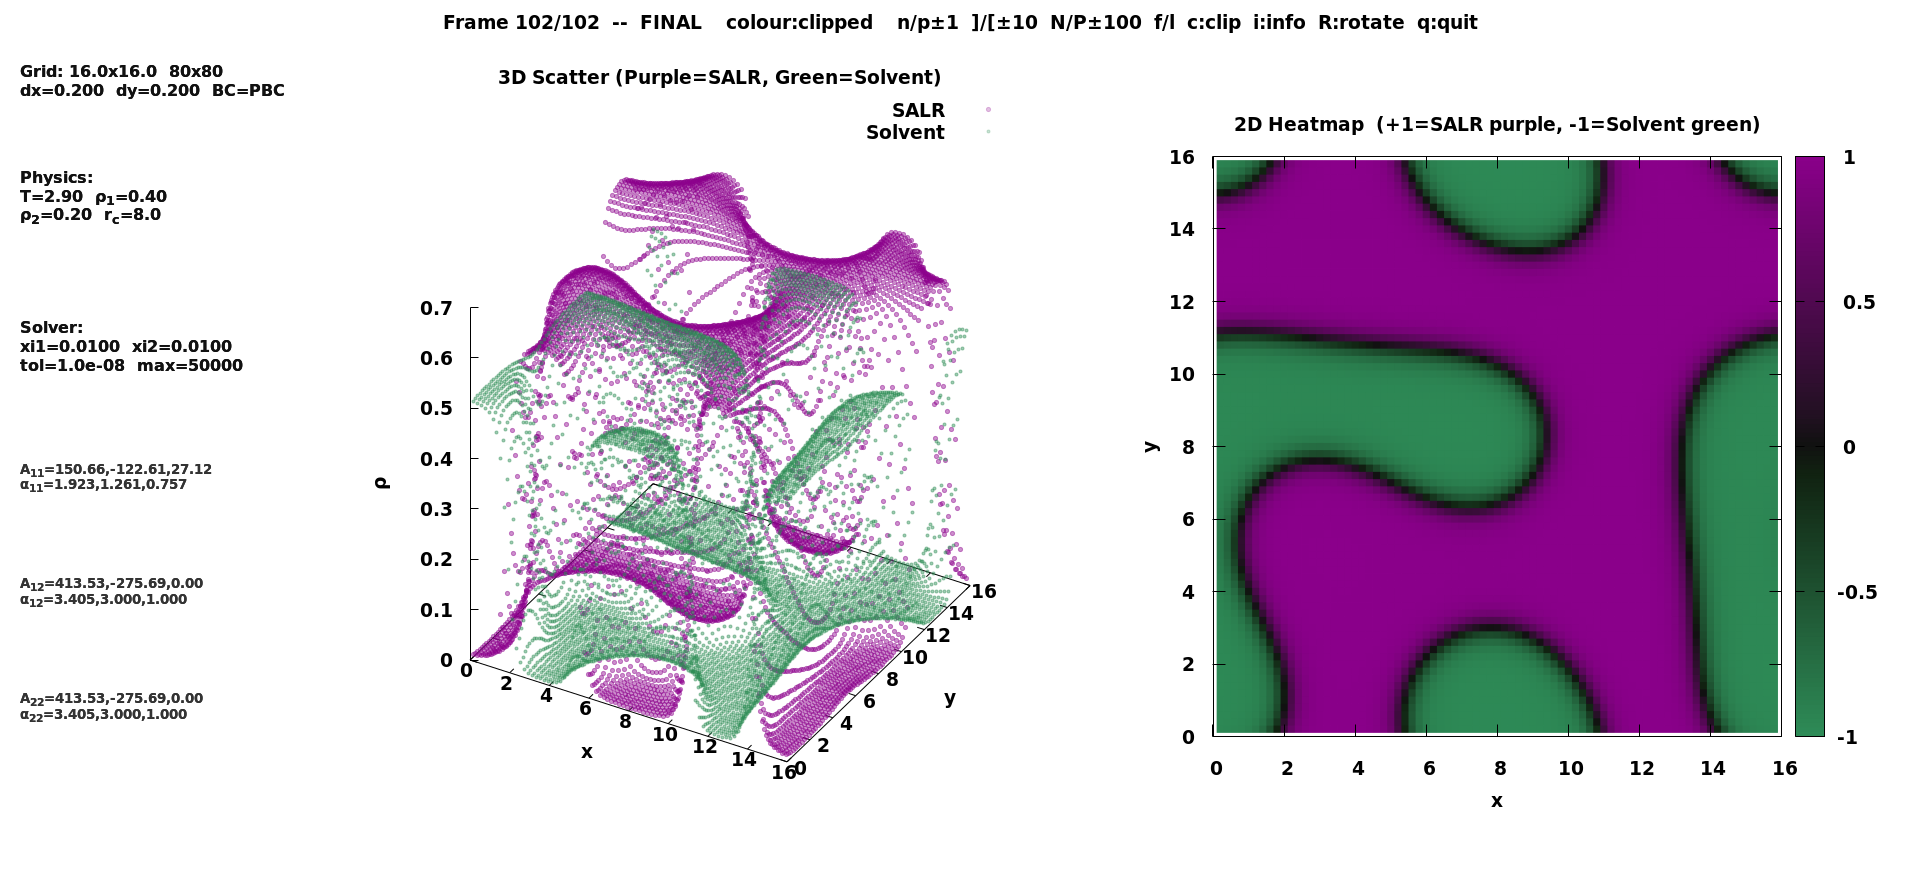
\includegraphics[width=0.92\columnwidth]{src/rep_pbc.png}}
\caption{Representative PBC snapshot (combined 2D and 3D view). Parameters shown in the image: $T=2.90$, $\rho_1=0.40$, $\rho_2=0.20$, $r_c=8.0$, grid $80\times80$ with $\Delta x=\Delta y=0.2$. Init mode not recorded.}
\label{fig:pbc_rep}
\end{figure}

\subsection{Two-Wall Confinement (W2)}

\subsubsection{Random starting distribution}

Under W2 confinement, the walls suppress density at $x=0$ and $x=L_x$, which drives the system toward wall-parallel modulation. Random starting distributions tend to produce uneven wall layers before relaxing into a more regular pattern.

\begin{figure}[htbp]
\centering
\fbox{\parbox{0.92\columnwidth}{\centering
\textbf{Placeholder}\\
Provide W2 random-start snapshot (combined 2D and 3D view).\\
File name: src/w2-random.png
}}
\caption{W2 with random starting distribution. Placeholder for a combined 2D and 3D snapshot.}
\label{fig:w2_random_placeholder}
\end{figure}

\subsubsection{Sinusoidal starting distribution}

With sinusoidal starting distributions, the solver tends to keep stripe orientation parallel to the walls, and the boundary layers stabilize faster due to the imposed spatial modulation.

\begin{figure}[htbp]
\centering
\fbox{\parbox{0.92\columnwidth}{\centering
\textbf{Placeholder}\\
Provide W2 sinusoidal-start snapshot (combined 2D and 3D view).\\
File name: src/w2-sinusoidal.png
}}
\caption{W2 with sinusoidal starting distribution. Placeholder for a combined 2D and 3D snapshot.}
\label{fig:w2_sinusoidal_placeholder}
\end{figure}

\subsubsection{Representative snapshot (init mode not recorded)}

Figure~\ref{fig:w2_rep} shows a representative W2 snapshot from the current results set. The init mode was not recorded in the snapshot, so it is shown here as an example of the boundary-driven morphology only. The parameter set matches the PBC representative snapshot.

\begin{figure}[htbp]
\centerline{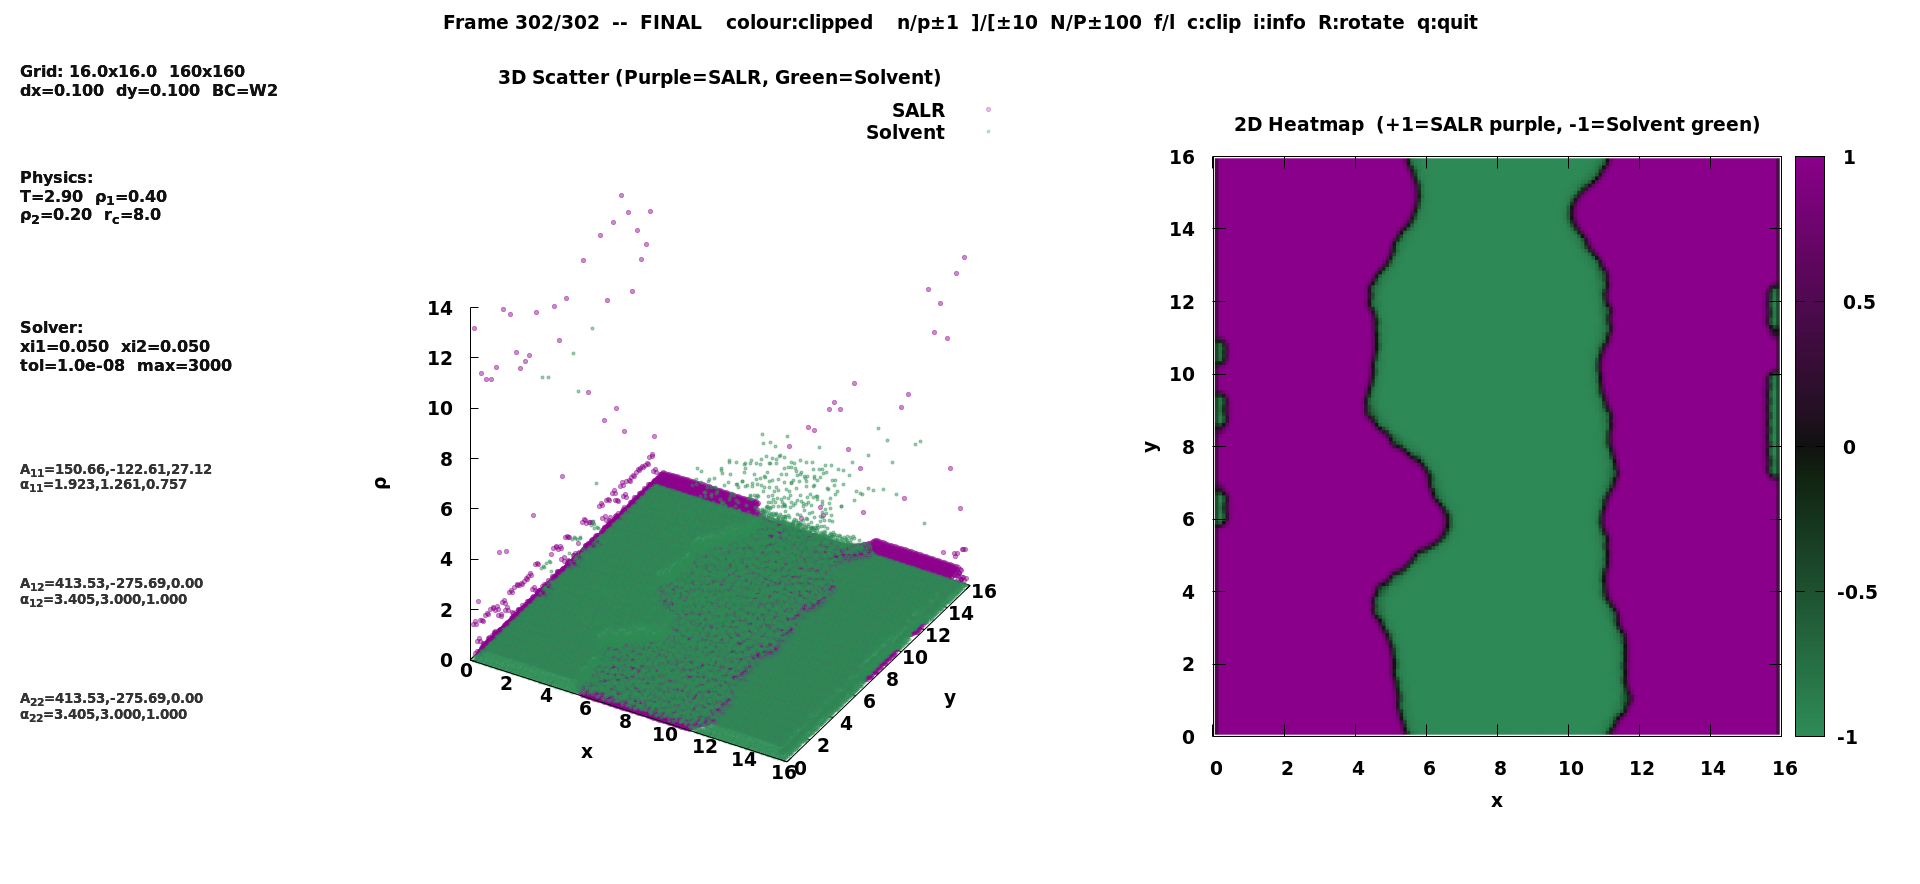
\includegraphics[width=0.92\columnwidth]{src/rep_w2.png}}
\caption{Representative W2 snapshot (combined 2D and 3D view). Parameters shown in the image: $T=2.90$, $\rho_1=0.40$, $\rho_2=0.20$, $r_c=8.0$, grid $160\times160$ with $\Delta x=\Delta y=0.1$. Init mode not recorded.}
\label{fig:w2_rep}
\end{figure}

\subsection{Four-Wall Confinement (W4)}

\subsubsection{Random starting distribution}

In the four-wall case, the random start often creates a dense core surrounded by a depleted boundary layer. Corner depletion becomes more pronounced as the field relaxes toward equilibrium.

\begin{figure}[htbp]
\centering
\fbox{\parbox{0.92\columnwidth}{\centering
\textbf{Placeholder}\\
Provide W4 random-start snapshot (combined 2D and 3D view).\\
File name: src/w4-random.png
}}
\caption{W4 with random starting distribution. Placeholder for a combined 2D and 3D snapshot.}
\label{fig:w4_random_placeholder}
\end{figure}

\subsubsection{Sinusoidal starting distribution}

For sinusoidal starts, the confined system tends to form a smoother central profile with stronger boundary depletion. The walls fix the pattern phase and reduce the number of competing domains.

\begin{figure}[htbp]
\centering
\fbox{\parbox{0.92\columnwidth}{\centering
\textbf{Placeholder}\\
Provide W4 sinusoidal-start snapshot (combined 2D and 3D view).\\
File name: src/w4-sinusoidal.png
}}
\caption{W4 with sinusoidal starting distribution. Placeholder for a combined 2D and 3D snapshot.}
\label{fig:w4_sinusoidal_placeholder}
\end{figure}

\subsubsection{Representative snapshot (init mode not recorded)}

Figure~\ref{fig:w4_rep} shows a representative W4 snapshot from the current results set. The init mode was not recorded in the snapshot, so it is shown here as an example of a confined morphology only. The parameter set matches the PBC representative snapshot.

\begin{figure}[htbp]
\centerline{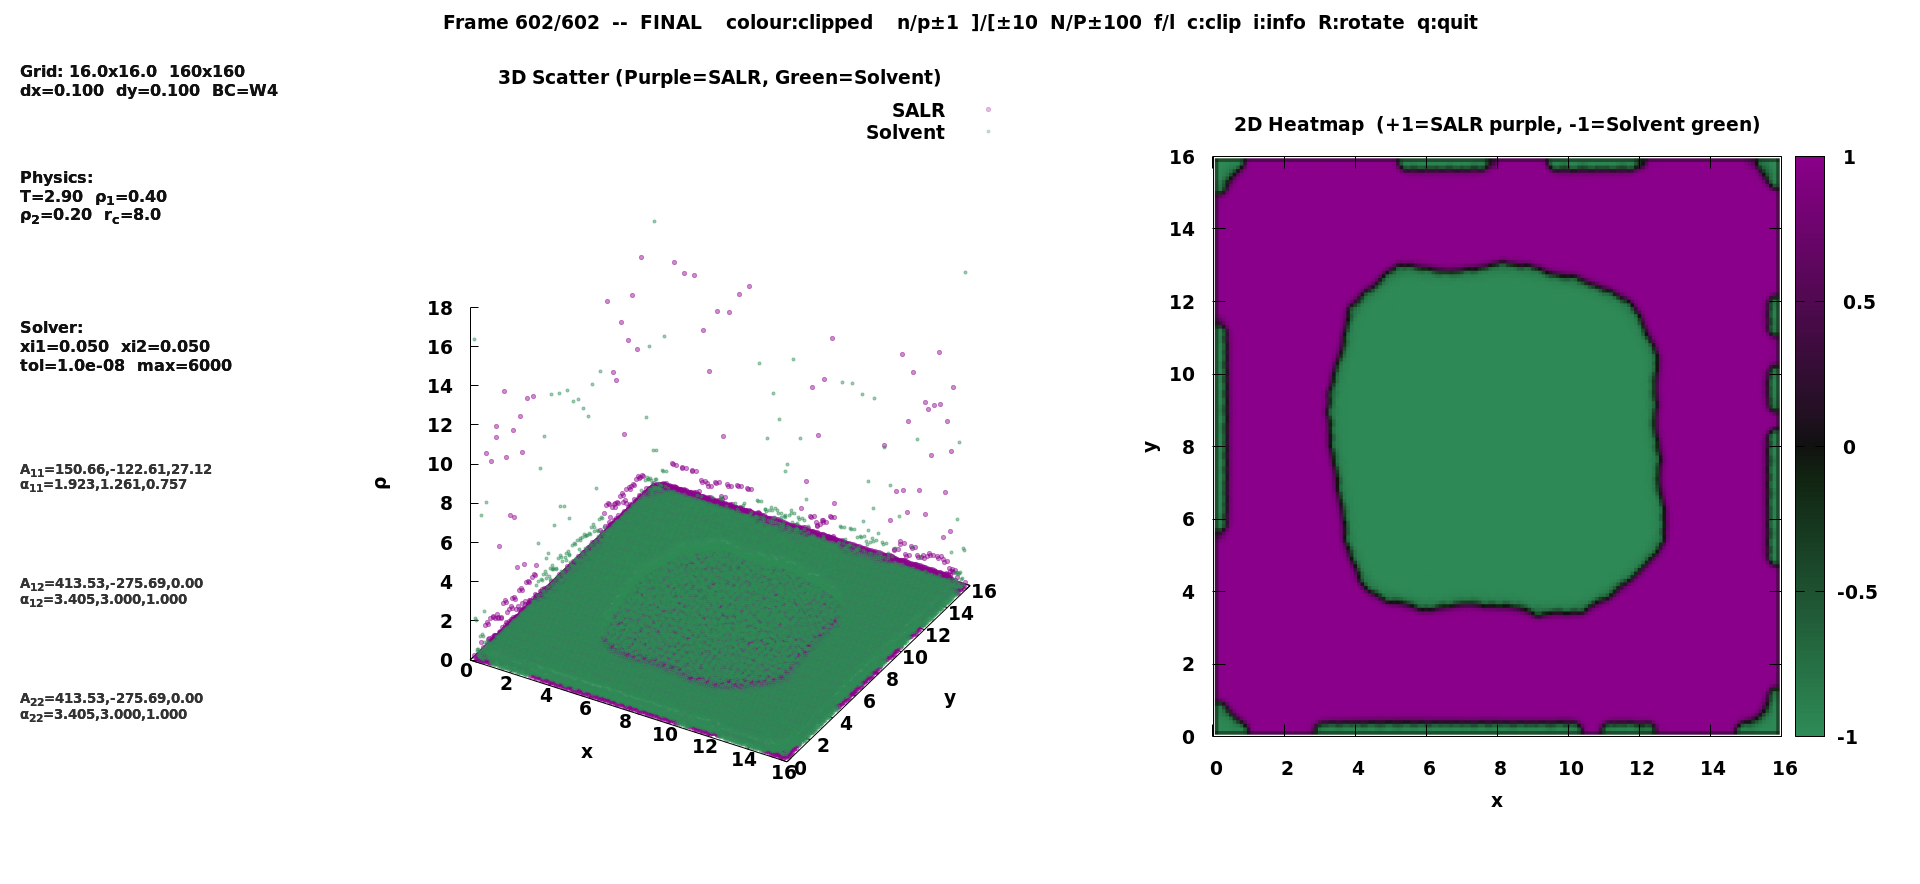
\includegraphics[width=0.92\columnwidth]{src/rep_w4.png}}
\caption{Representative W4 snapshot (combined 2D and 3D view). Parameters shown in the image: $T=2.90$, $\rho_1=0.40$, $\rho_2=0.20$, $r_c=8.0$, grid $160\times160$ with $\Delta x=\Delta y=0.1$. Init mode not recorded.}
\label{fig:w4_rep}
\end{figure}

\subsection{Performance on our Machines}

\subsubsection{Measured metrics}

We focus on two primary metrics: wall time per run and speedup. Speedup is reported as $S = t_{CPU} / t_{CUDA}$ or relative to a single CPU thread when comparing OpenMP scaling.

\subsubsection{Benchmark parameters and hardware}

The performance benchmarks use the dedicated benchmark configuration (I/O disabled) with the same physical parameters as the default solver configuration. Grid sizes and thread counts follow the measured dataset from the laptop benchmark logs:

\begin{itemize}
    \item Grid sizes: $N \in \{16, 32, 64, 128, 160, 256, 320\}$.
    \item CPU threads: $\{1, 2, 4, 8, 12, 16, 20\}$ and CUDA on the GPU.
    \item Max iterations: $1000$, tolerance $10^{-8}$, boundary mode PBC, init mode sinusoids.
\end{itemize}

Laptop hardware used for the benchmark run is summarized in Table~\ref{tab:laptop_hw}. Several low-level hardware properties were not captured in the logs and are left as placeholders.

\begin{table}[htbp]
\caption{Laptop hardware used for benchmarks}
\begin{center}
\begin{tabular}{|l|l|}
\hline
\textbf{Parameter} & \textbf{Value} \\
\hline
CPU model & Intel Core i7-13700H \\
CPU cores or threads & 20 threads \\
CPU frequency & TODO \\
CPU cache (L1, L2, L3) & TODO \\
RAM size and type & TODO \\
GPU model & NVIDIA GeForce RTX 4060 Laptop GPU \\
GPU architecture & TODO \\
GPU core count & TODO \\
GPU clock speed & TODO \\
VRAM capacity & 8188 MiB \\
VRAM type and bus width & TODO \\
Memory bandwidth & TODO \\
Throughput (TFLOPS) & TODO \\
GPU cache levels & TODO \\
\hline
\end{tabular}
\label{tab:laptop_hw}
\end{center}
\end{table}

\subsubsection{Methodology}

Each $(N, \text{threads})$ configuration was executed three times, and the benchmark script wrote the aggregated wall time to CSV. Disk I/O was disabled via a large save interval to ensure timing reflects compute only. CUDA and CPU runs use the same grid and physical parameters.

\subsubsection{Benchmark results}

Figure~\ref{fig:laptop_perf} reports execution time versus grid size for all CPU thread counts and CUDA. CUDA is slower for the smallest grid ($N=16$) due to launch overheads, but becomes faster from $N=32$ onward. At $N=160$, CUDA is about $5.0\times$ faster than the 20-thread CPU run. CPU timing for $N=256$ and $N=320$ is not recorded in the benchmark logs, so those points appear only for CUDA.

Figure~\ref{fig:laptop_speedup} shows CUDA speedup versus each CPU baseline and the CPU parallel scaling relative to a single thread. CPU speedup saturates near $7$ to $8\times$ at the largest grid sizes, indicating memory bandwidth and synchronization limits.

The convergence check in Figure~\ref{fig:laptop_real_params} confirms that CPU and CUDA reach the same tolerance and iteration count for the default physical parameters.

\begin{figure}[htbp]
\centerline{
\includegraphics[width=\columnwidth]{src/performance_comparison.png}}
\caption{Laptop benchmark runtime for CUDA and CPU across grid sizes.}
\label{fig:laptop_perf}
\end{figure}

\begin{figure}[htbp]
\centerline{
\includegraphics[width=\columnwidth]{src/speedup_analysis.png}}
\caption{Laptop benchmark speedups: CUDA over CPU (left) and CPU OpenMP scaling (right).}
\label{fig:laptop_speedup}
\end{figure}

\begin{figure}[htbp]
\centerline{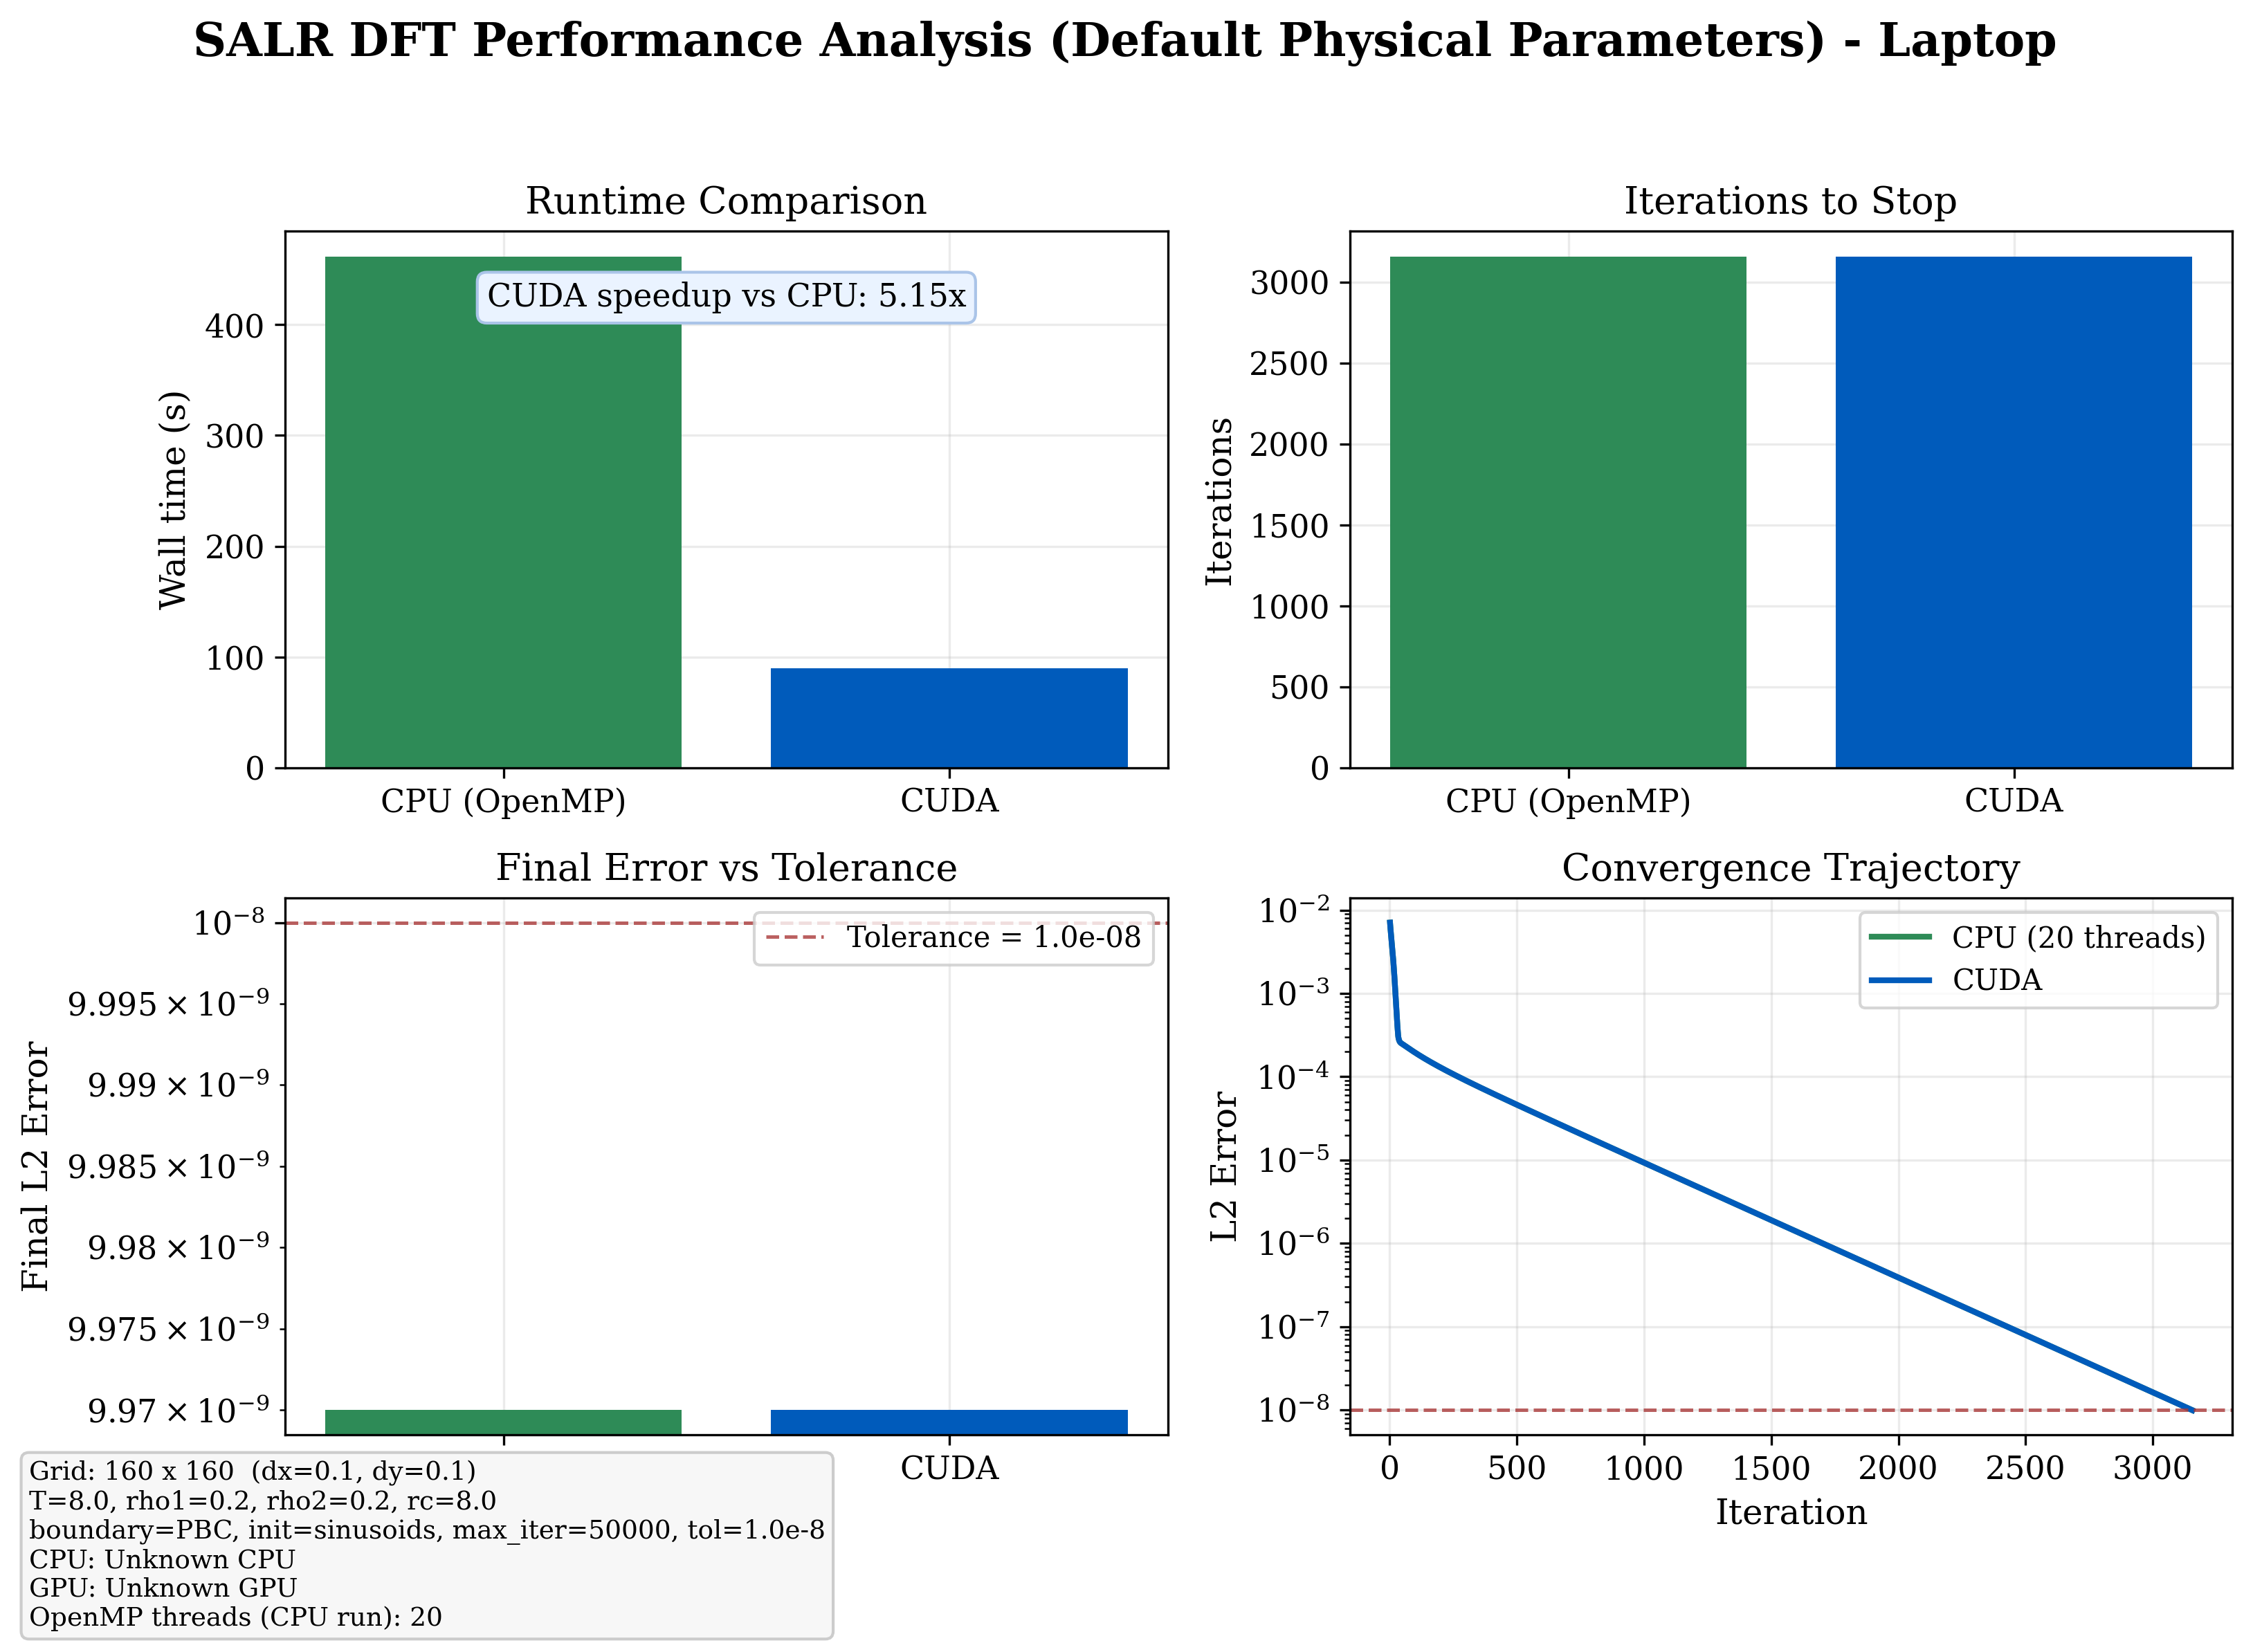
\includegraphics[width=\columnwidth]{src/performance_real_params_laptop.png}}
\caption{Laptop convergence comparison for default physical parameters. CPU and CUDA converge to the same error threshold with identical iteration counts.}
\label{fig:laptop_real_params}
\end{figure}

\subsection{Missing assets}

The following images are required to complete the random and sinusoidal starting condition sections. Once added, replace the placeholders above and remove this list.

\begin{itemize}
    \item src/pbc-random.png
    \item src/pbc-sinusoidal.png
    \item src/w2-random.png
    \item src/w2-sinusoidal.png
    \item src/w4-random.png
    \item src/w4-sinusoidal.png
\end{itemize}

%--------------------------
\section{Results on Cluster}
%--------------------------

\subsection{Benchmark setup}

Cluster benchmarks use the same benchmark configuration as the laptop run, with I/O disabled and $1000$ iterations per configuration. The dataset contains three machine classes:

\begin{itemize}
    \item AMD EPYC 9754 (CPU only, no NVIDIA GPU detected).
    \item AMD Threadripper PRO 5975WX (CPU only, no NVIDIA GPU detected).
    \item AMD Threadripper PRO 5975WX with NVIDIA GeForce RTX 5090.
\end{itemize}

All benchmark CSV files record the same grid sizes ($N=16$ to $160$). EPYC thread counts include $\{1, 2, 4, 8, 16, 32, 64\}$, while the Threadripper datasets include $\{1, 2, 4, 8, 16\}$. The EPYC dataset does not include a 1-thread measurement at $N=160$.

\subsection{Hardware summary}

Cluster hardware details captured by the benchmark logs are summarized in Table~\ref{tab:cluster_hw}. Additional properties such as cache sizes, memory types, and GPU bandwidth were not recorded and remain to be filled.

\begin{table*}[t]
\caption{Cluster hardware used for benchmarks}
\label{tab:cluster_hw}
\begin{center}
\begin{tabularx}{\textwidth}{|l|X|c|l|c|}
\hline
\textbf{Node} & \textbf{CPU model} & \textbf{Cores} & \textbf{GPU} & \textbf{VRAM} \\
\hline
EPYC node & AMD EPYC 9754 & 256 & None & N/A \\
\hline
Threadripper CPU & AMD Threadripper PRO 5975WX & 32 & None & N/A \\
\hline
Threadripper GPU & AMD Threadripper PRO 5975WX & 32 & NVIDIA GeForce RTX 5090 & 32607 MiB \\
\hline
\end{tabularx}
\end{center}
\end{table*}

\subsection{Performance across cluster nodes}

Figure~\ref{fig:cluster_cpu_log} compares the best CPU time per grid size across laptop and cluster nodes. Figure~\ref{fig:cluster_thread_speedup} summarizes OpenMP scaling at the largest measured grid size. Figures~\ref{fig:cluster_gpu_runtime} and~\ref{fig:cluster_speedup} show GPU versus CPU performance and speedup relative to the laptop baseline.

\begin{figure}[htbp]
\centerline{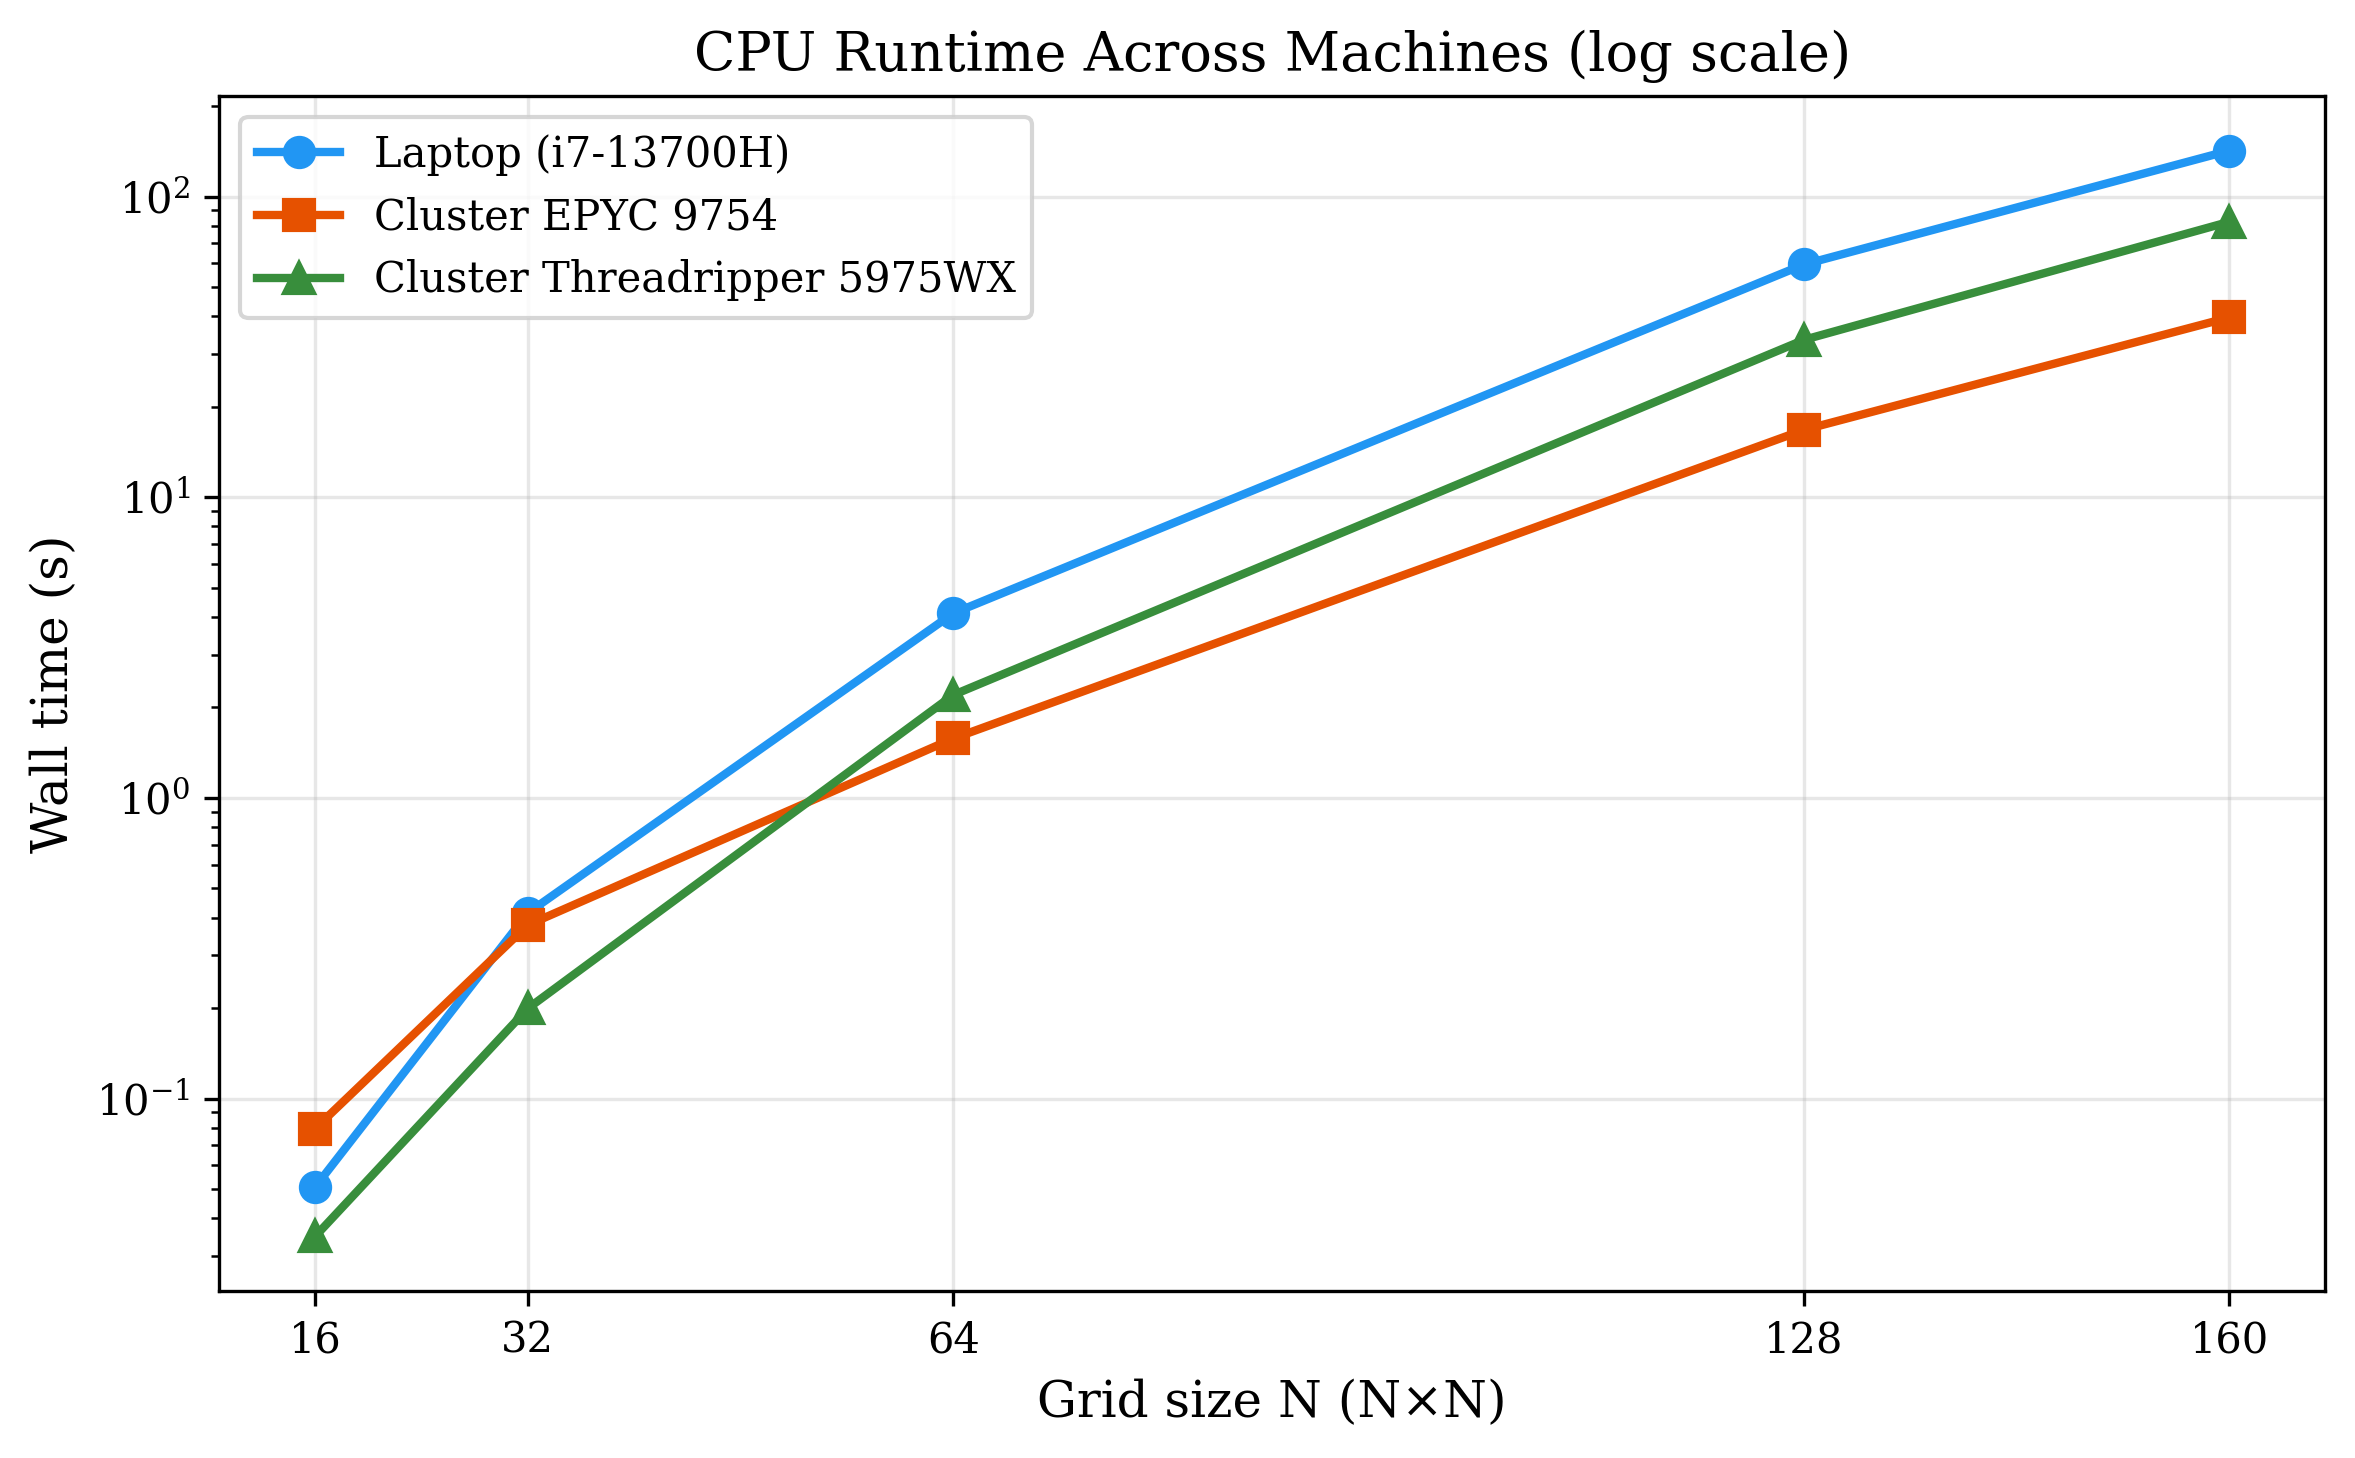
\includegraphics[width=\columnwidth]{src/cpu_runtime_log.png}}
\caption{Best CPU runtime across laptop and cluster machines (log scale).}
\label{fig:cluster_cpu_log}
\end{figure}

\begin{figure}[htbp]
\centerline{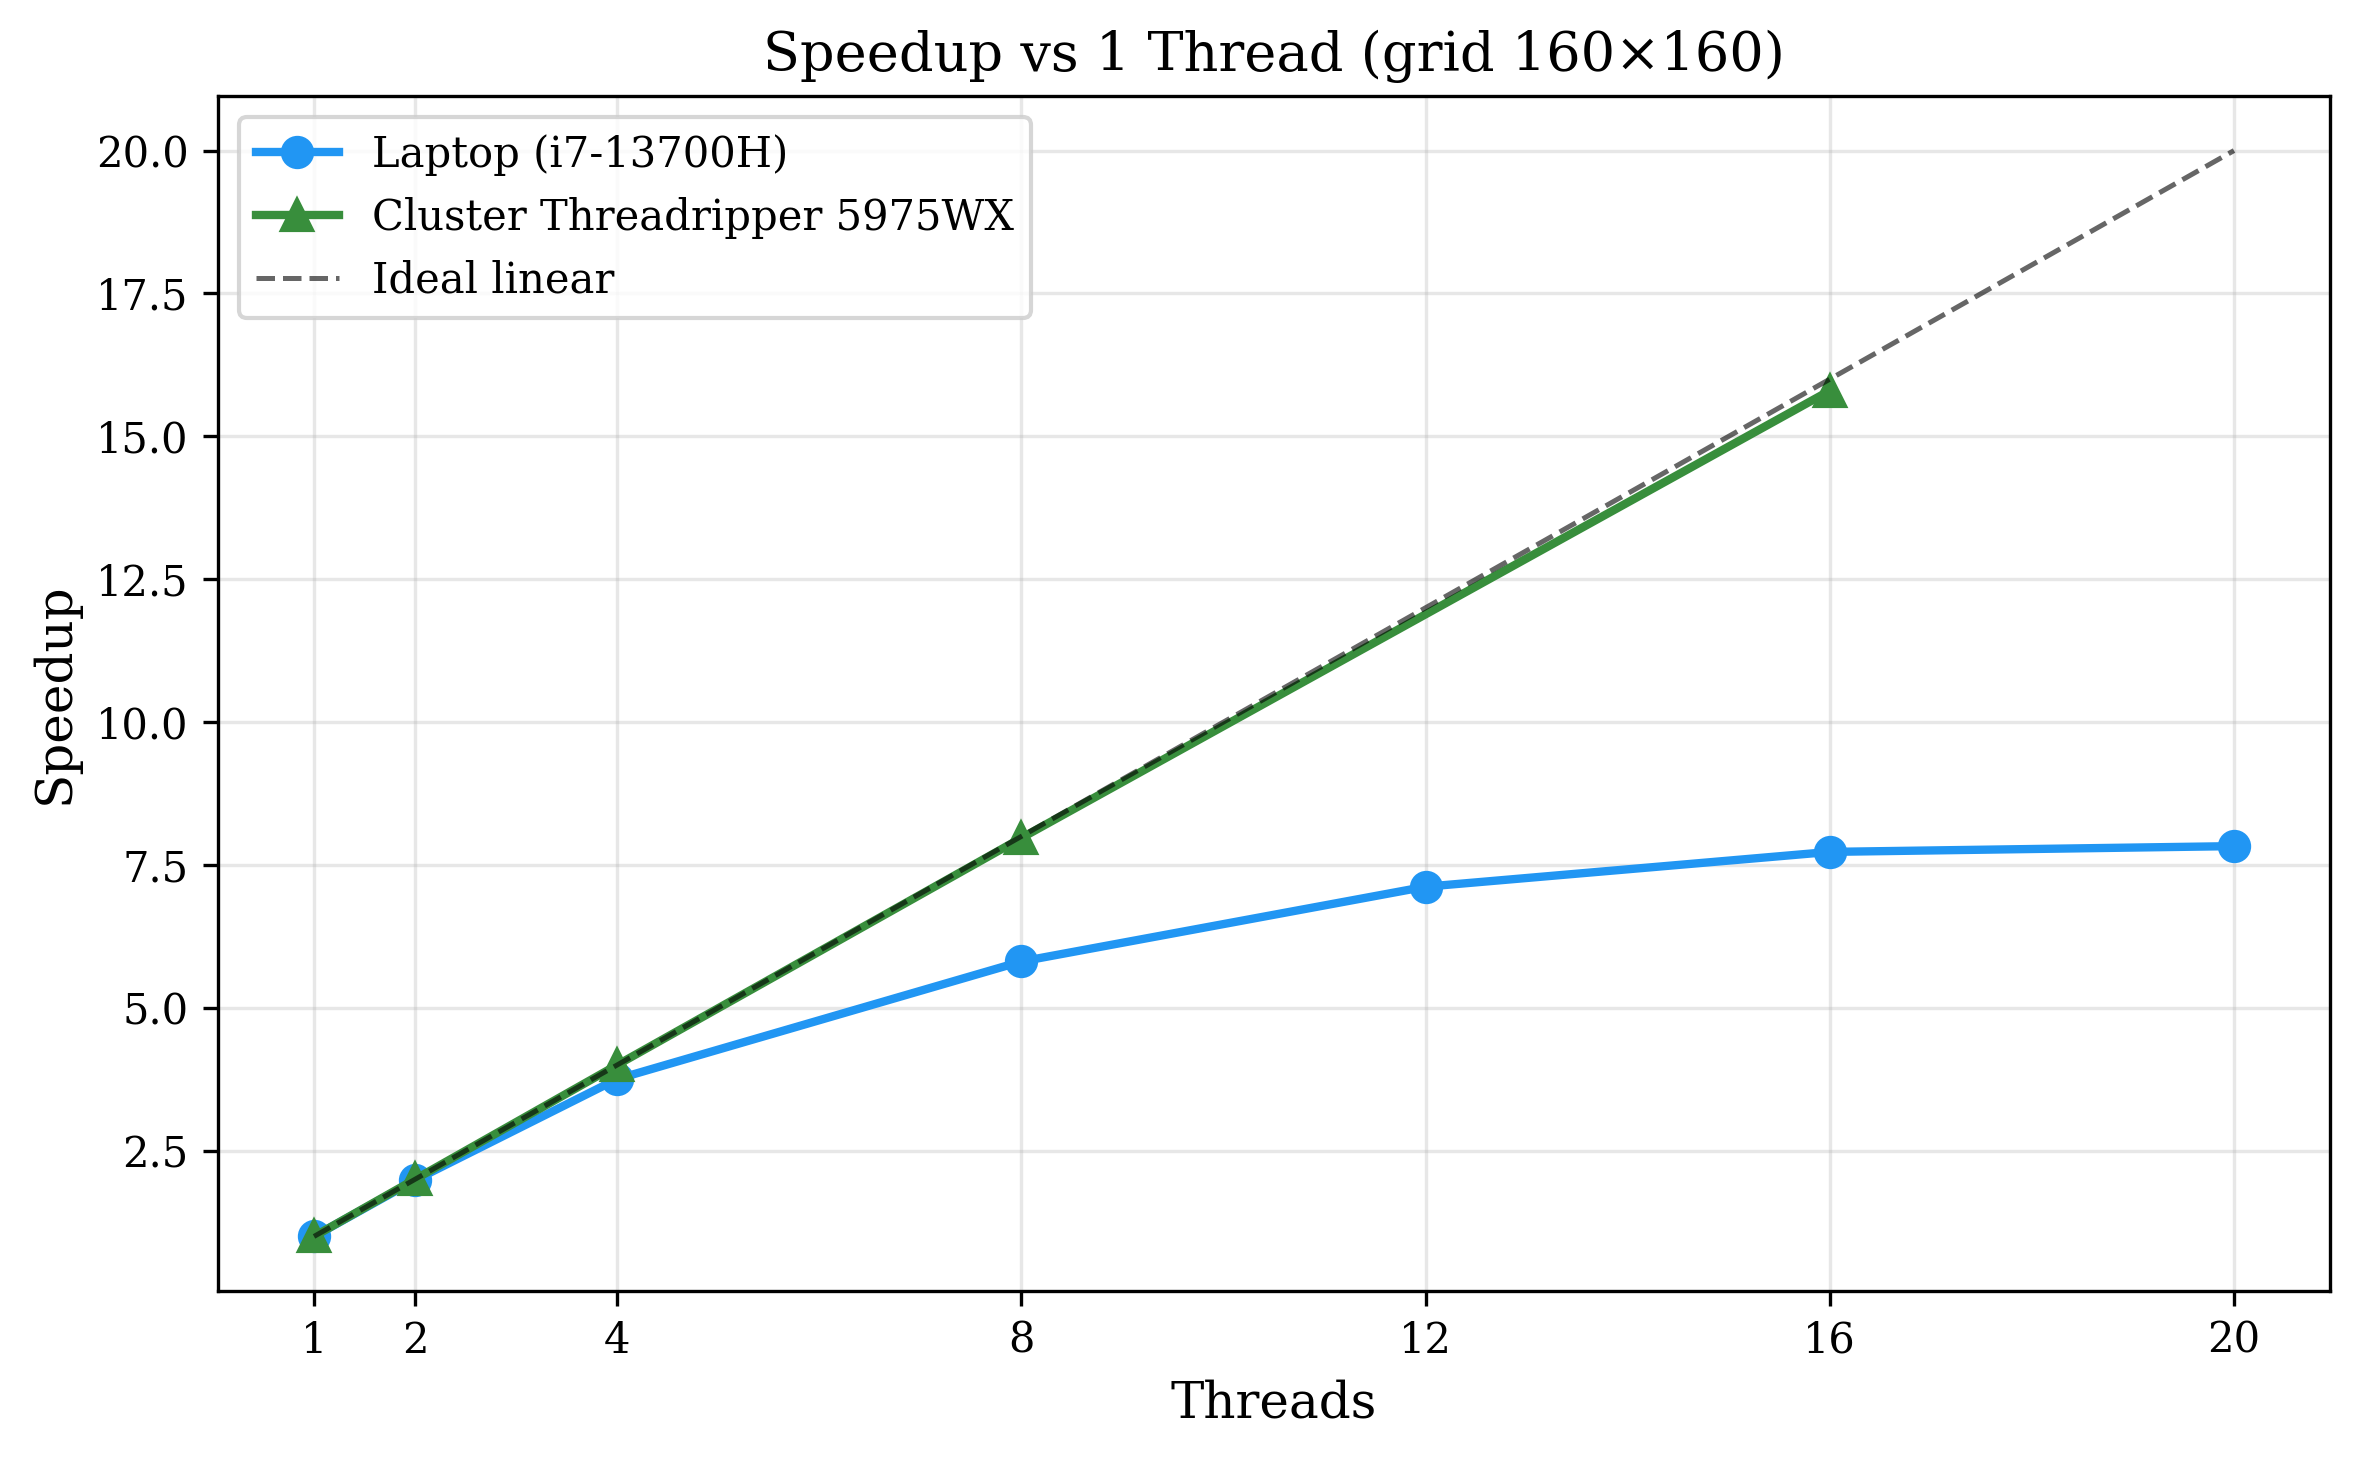
\includegraphics[width=\columnwidth]{src/thread_scaling_speedup.png}}
\caption{OpenMP speedup versus single-thread baseline for the largest available grid size.}
\label{fig:cluster_thread_speedup}
\end{figure}

\begin{figure}[htbp]
\centerline{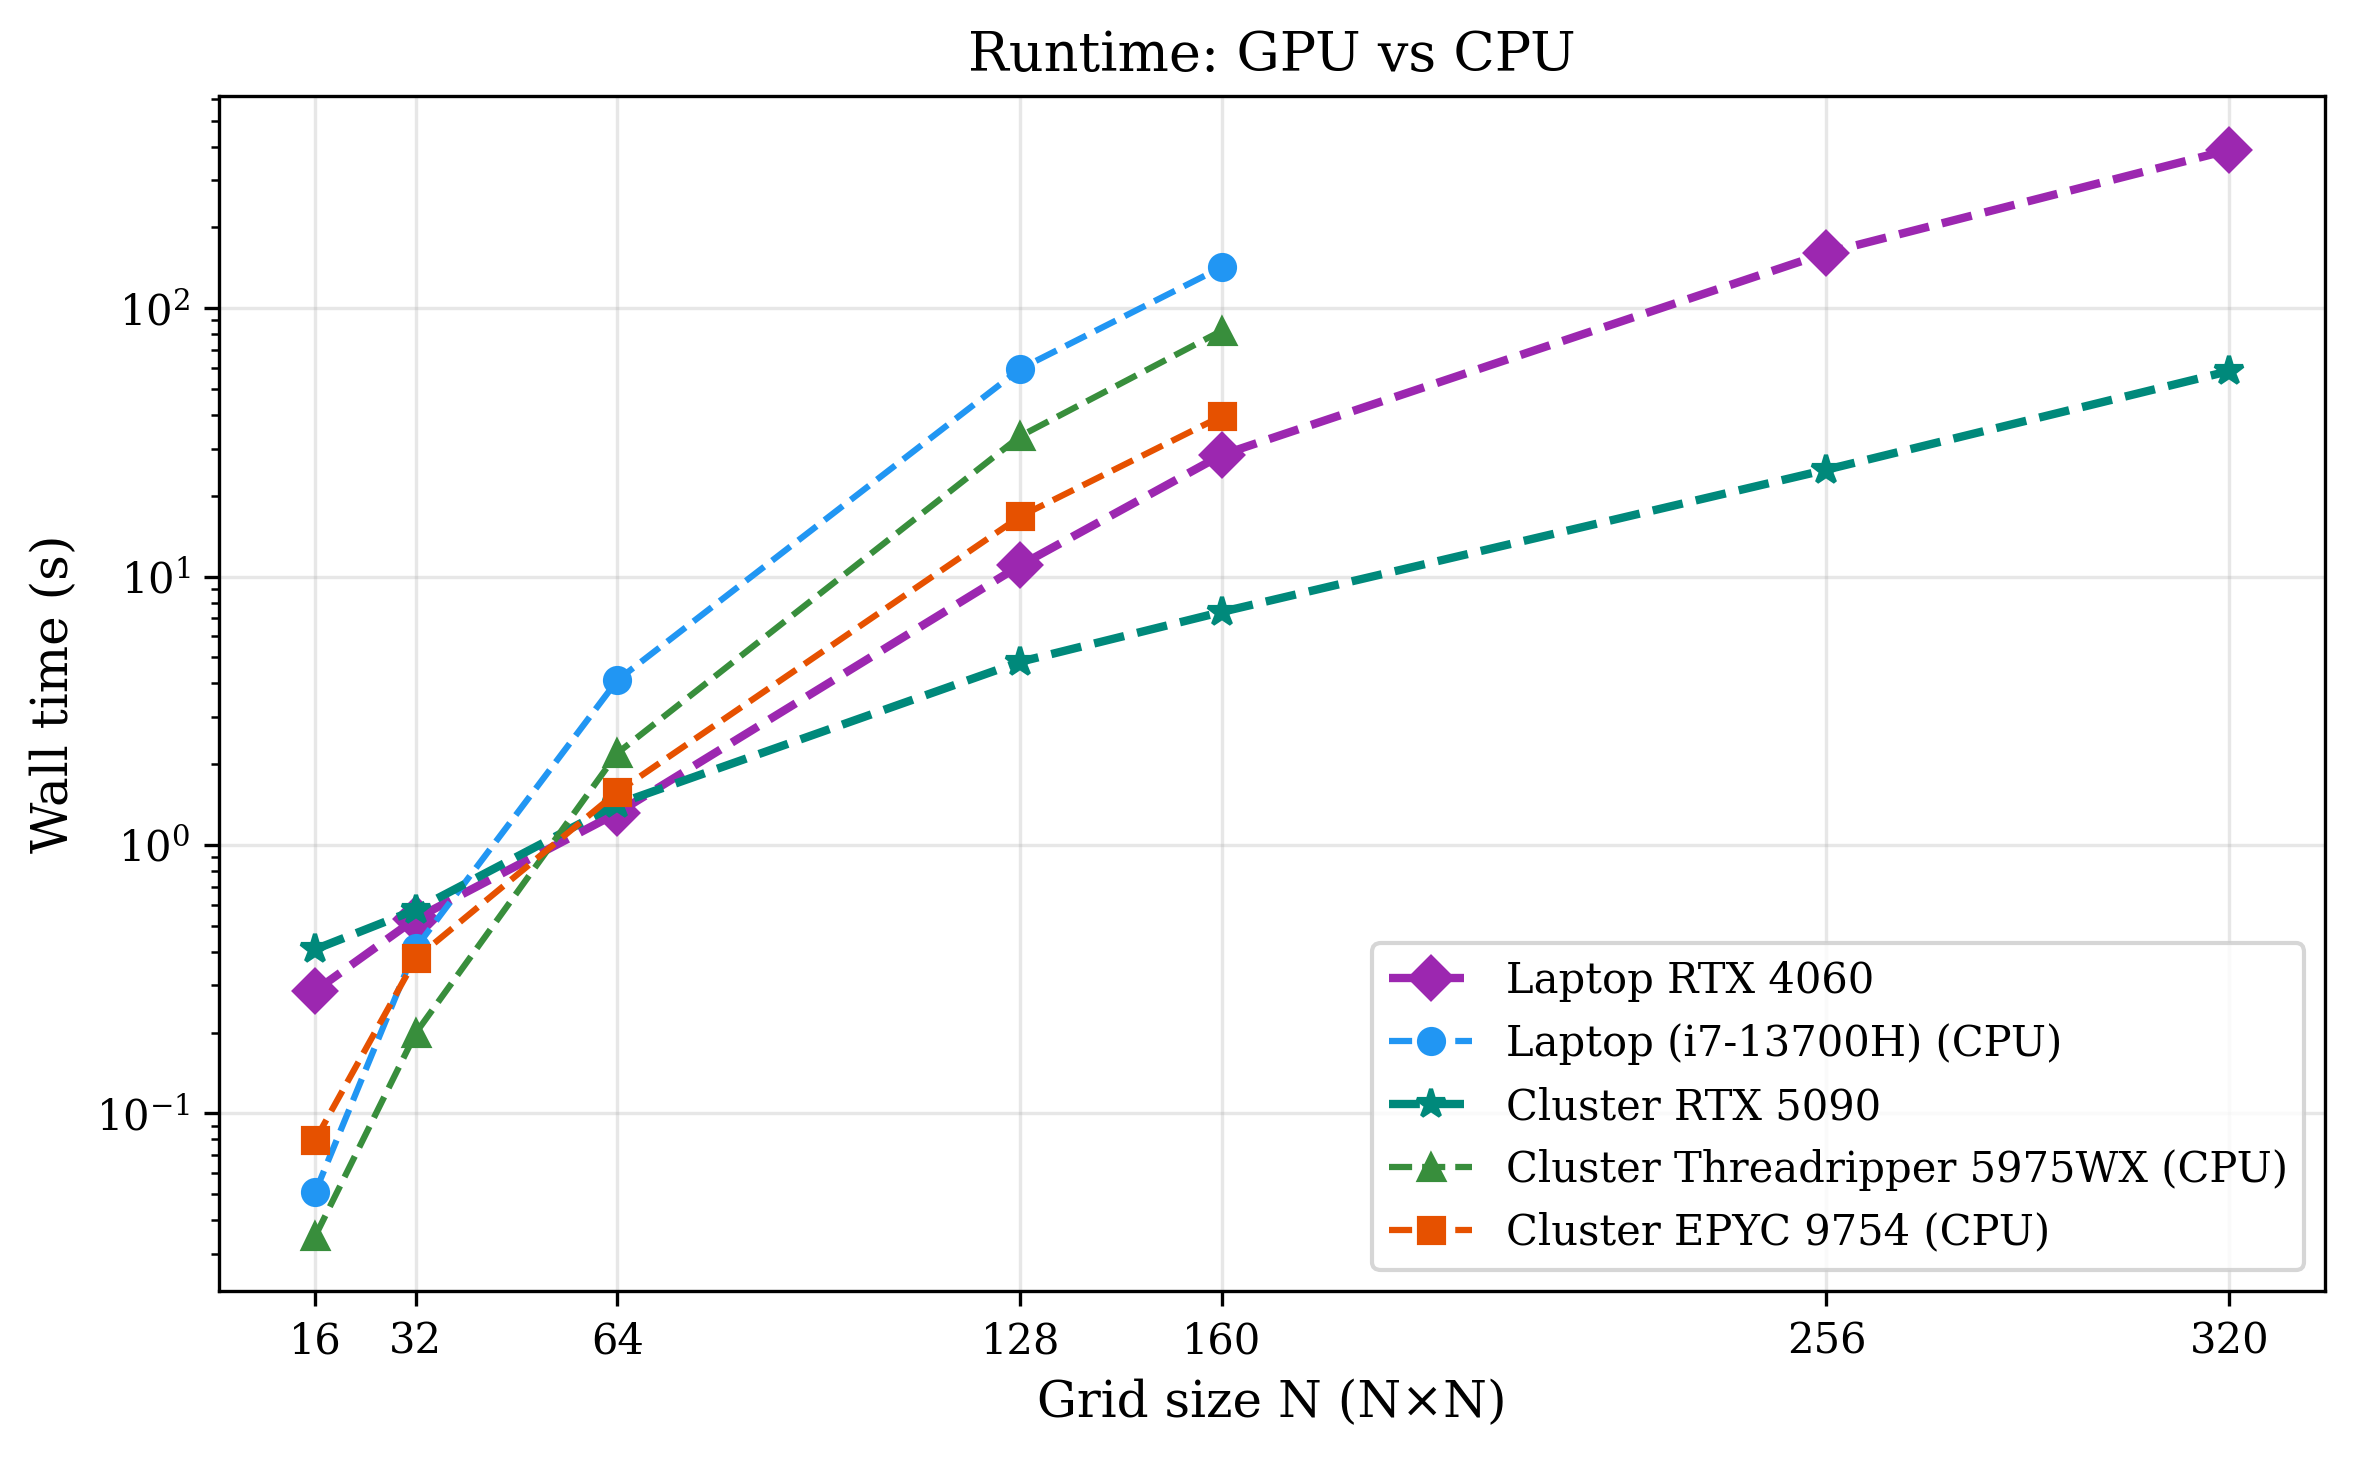
\includegraphics[width=\columnwidth]{src/gpu_runtime.png}}
\caption{GPU and CPU runtime comparison across machines. CPU-only nodes are shown without GPU curves.}
\label{fig:cluster_gpu_runtime}
\end{figure}

\begin{figure}[htbp]
\centerline{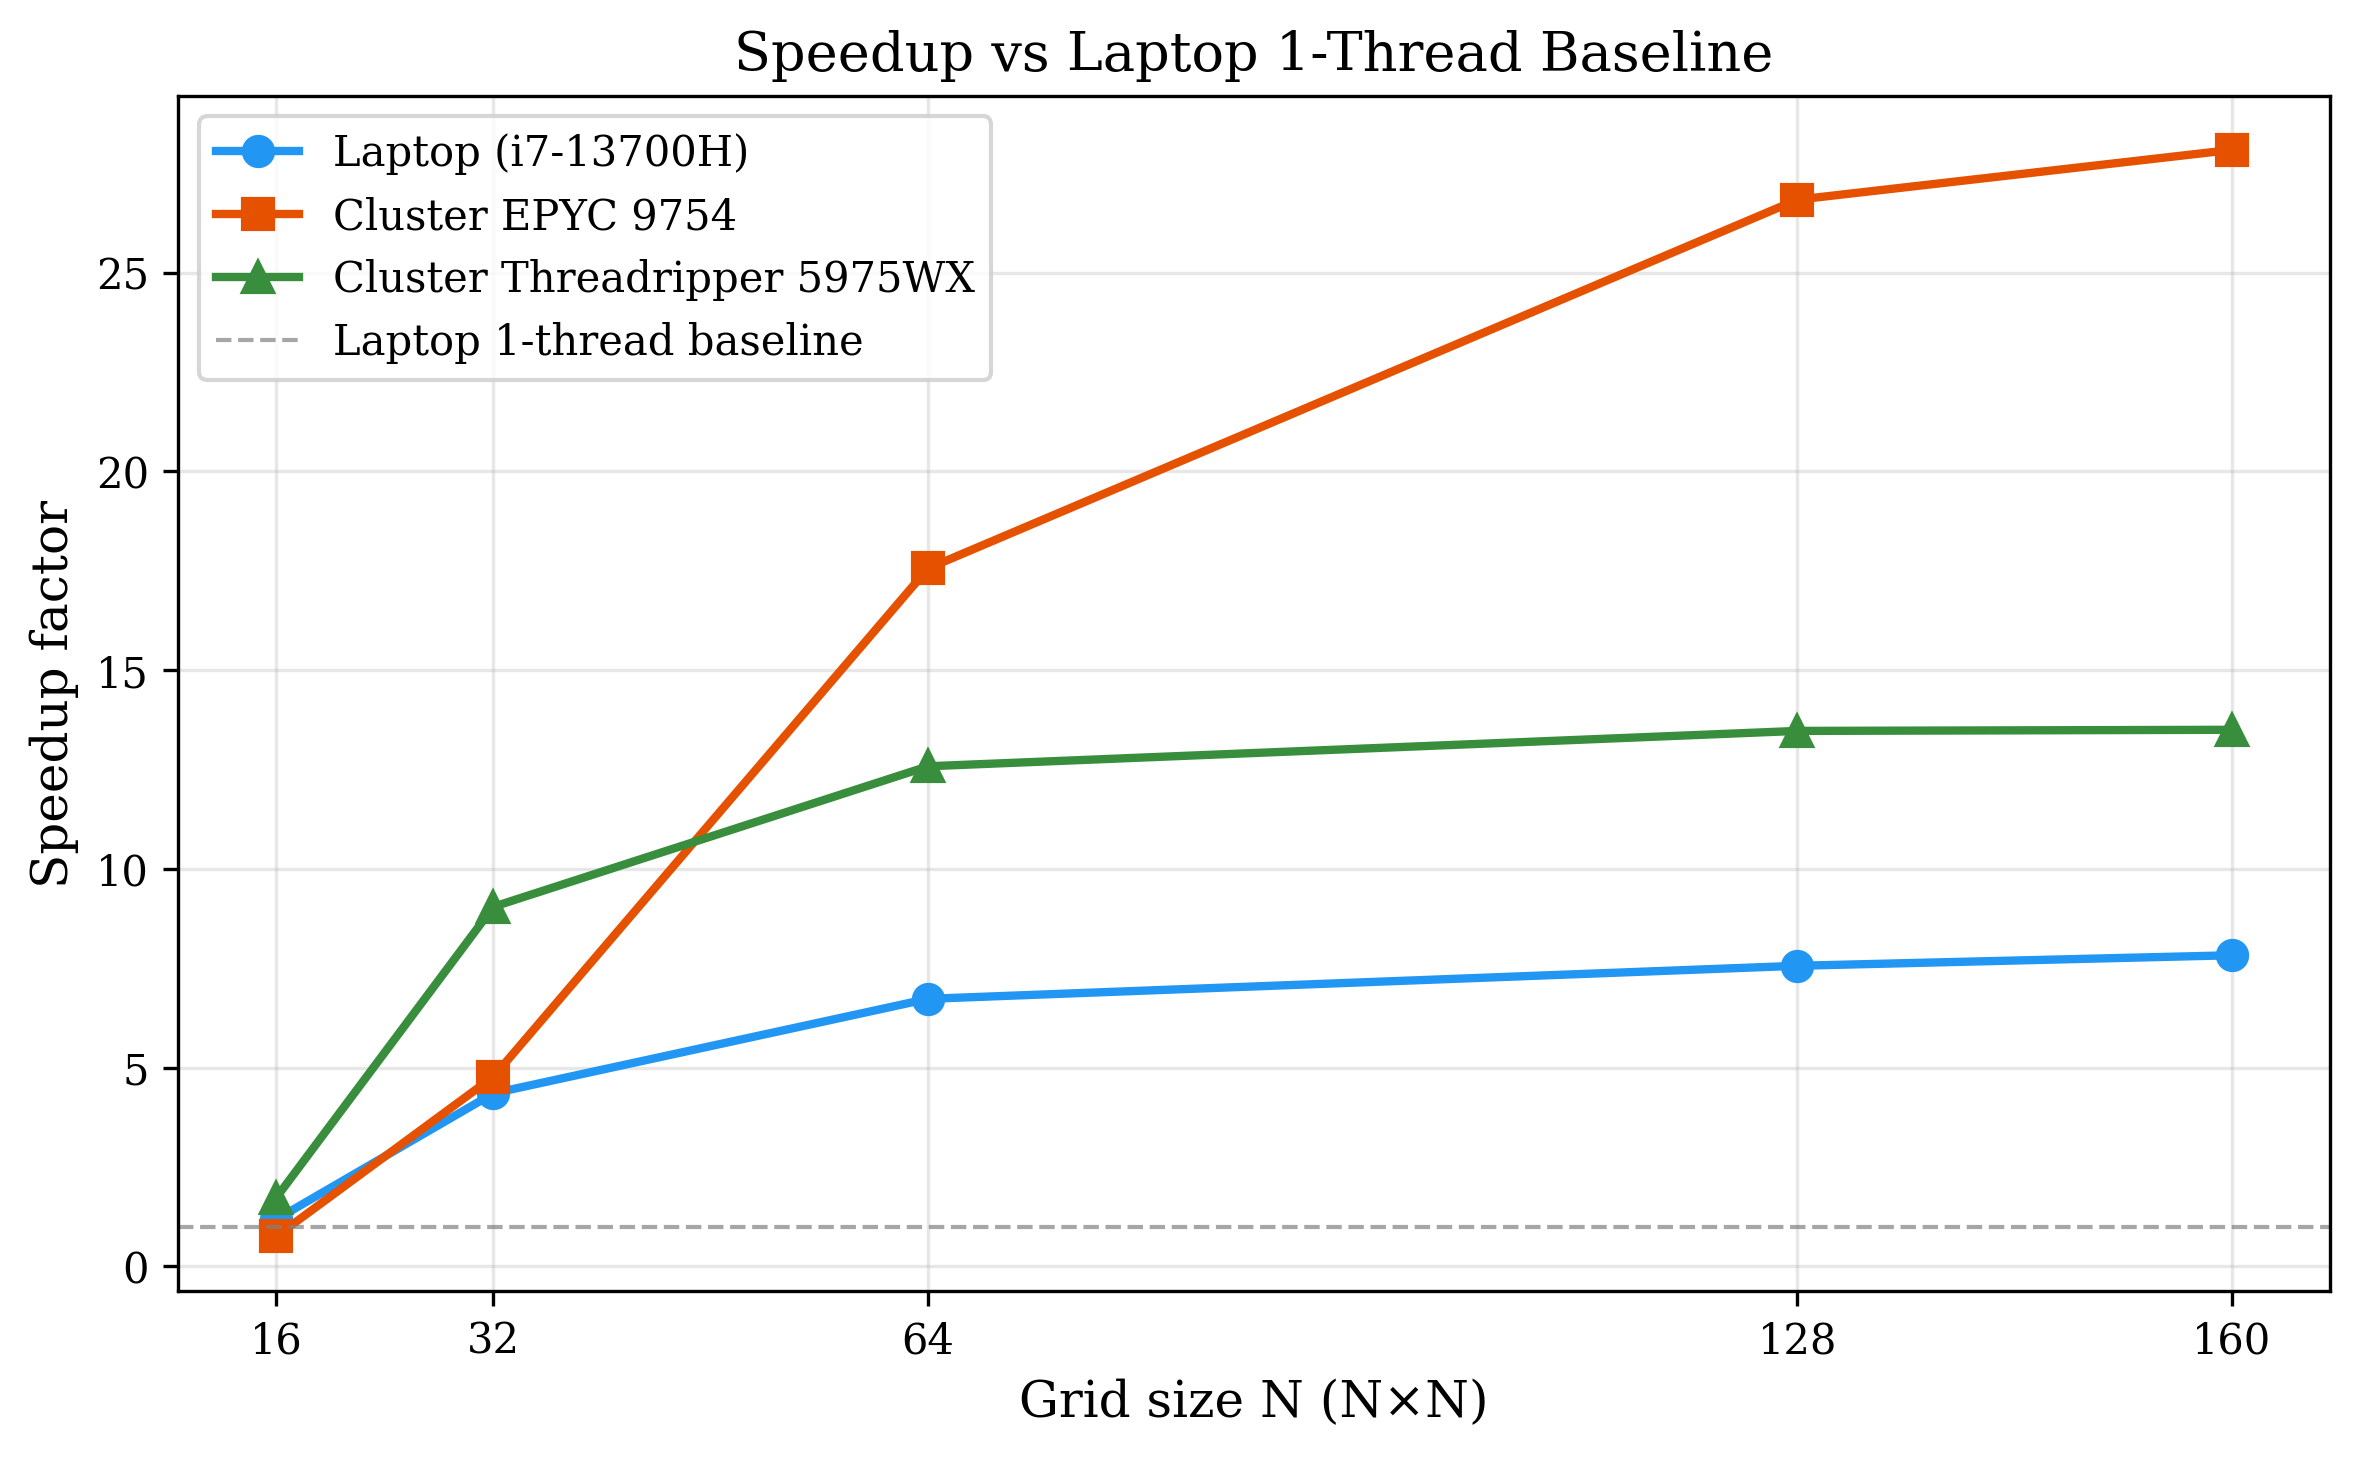
\includegraphics[width=\columnwidth]{src/speedup_vs_laptop.png}}
\caption{Speedup of each machine relative to the laptop single-thread baseline.}
\label{fig:cluster_speedup}
\end{figure}

\subsection{Convergence check on the cluster GPU}

Figure~\ref{fig:cluster_real_params} summarizes the convergence comparison for the RTX 5090 run with a single-thread CPU baseline. The iteration counts and final error match, confirming numerical equivalence between CPU and CUDA implementations.

\begin{figure}[htbp]
\centerline{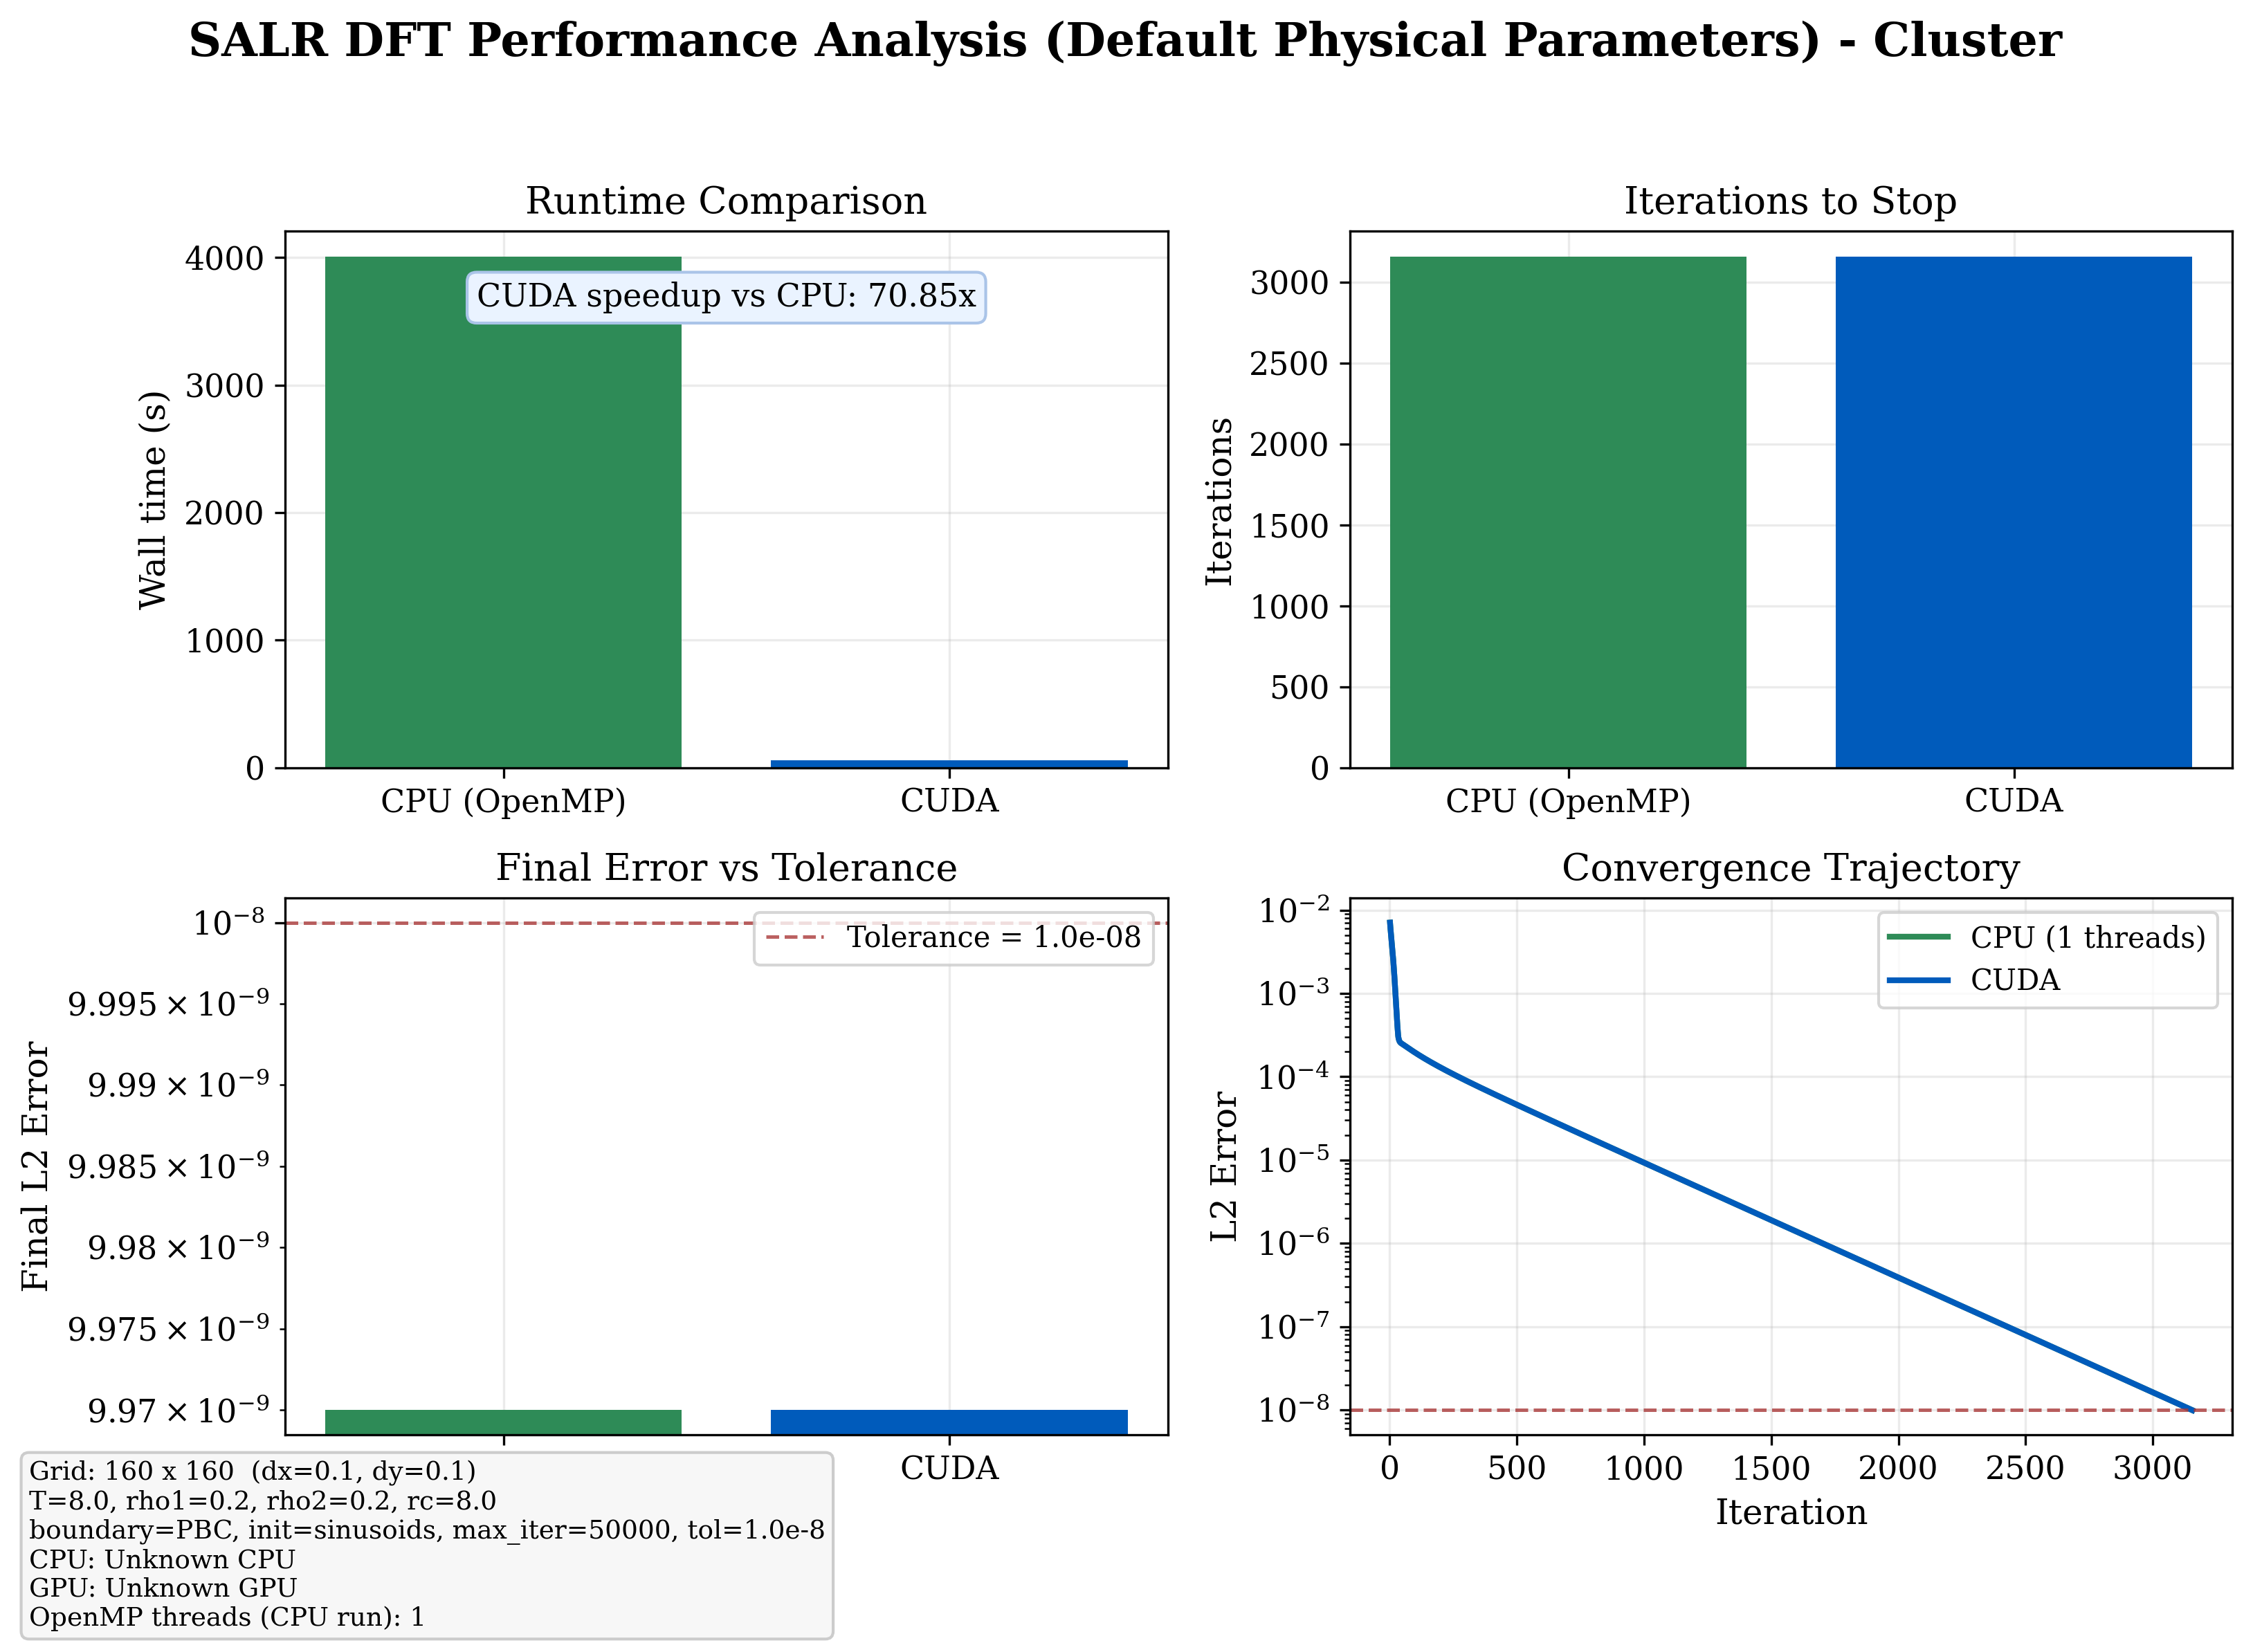
\includegraphics[width=\columnwidth]{src/performance_real_params_cluster.png}}
\caption{Cluster convergence comparison for default physical parameters (Threadripper PRO 5975WX with RTX 5090).}
\label{fig:cluster_real_params}
\end{figure}

%--------------------------
\section{Discussion}
%--------------------------

The computed density distributions demonstrate that our solver captures the essential physics of SALR systems: microphase separation driven by competing interactions, and the influence of confinement on pattern morphology. The results also confirm that initial conditions can steer the solver toward distinct local minima. Random starts frequently generate chaotic structures, while sinusoidal starts stabilize diagonal stripes more reliably.

At low temperatures, the density field can develop point-like spikes that appear gradually during iteration. We do not yet know whether these are physical microstructures or numerical artifacts, but their presence suggests that additional verification is required for low $T$ runs.

In the direct integration algorithm, we observed accumulation of numerical error that drives the solution toward near-zero uniform density or produces inf and NaN values. Adding normalization and Laplace smoothing mitigates most failures, but the result remains sensitive to the smoothing coefficient, so it must be tuned carefully.

Performance data highlight the benefits of GPU acceleration and the limits of CPU scaling. On the laptop, CUDA is slower only for the smallest grid ($N=16$), then surpasses all CPU thread counts for larger grids and reaches about a $5.0\times$ speedup at $N=160$. On the cluster RTX 5090 run, the CUDA solver achieves a $70.85\times$ speedup over a single-thread CPU baseline for the same physical parameters. CPU speedup saturates near $7$ to $8\times$ at the largest grids, indicating bandwidth and synchronization bottlenecks.

%--------------------------
\section{Conclusion}
%--------------------------

We have presented SALR3YUCUDA, a computational solver for mean-field DFT equations describing binary SALR colloidal mixtures. The CPU implementation with OpenMP parallelization and the CUDA accelerator both compute equilibrium density distributions under periodic and confined boundary conditions, capturing the stripe-like morphologies expected for competing interactions.

The benchmark set shows that GPU acceleration provides substantial gains. For the laptop dataset, CUDA reaches convergence about $5.15\times$ faster than the 20-thread CPU baseline for the default physical parameters. On the cluster RTX 5090 run, CUDA delivers a $70.85\times$ speedup over a single-thread CPU baseline. The integrated Qt GUI serves as a practical pipeline for iterative testing and on-the-fly visualization of distributions.

Future work will expand horizontally along several vectors including:
\begin{itemize}
    \item Extension to true three-dimensional domains.
    \item Multi-GPU scaling via deep domain decomposition.
    \item Automated phase-diagram extraction algorithms mapping extensive structural regions seamlessly across the interactive GUI.
\end{itemize}

%--------------------------
\section*{Acknowledgment}
%--------------------------

This work was performed as part of the Architecture of Computer Systems course at Ukrainian Catholic University. We thank the course instructors for guidance on parallelization strategies.

%--------------------------
\begin{thebibliography}{00}

\bibitem{royall2018}
C.~P. Royall, ``Hunting mermaids in real space: known knowns, known unknowns and unknown unknowns,'' \textit{Soft Matter}, vol.~14, no.~20, pp.~4020--4028, 2018.

\bibitem{liu2019}
Y.~Liu and Y.~Xi, ``Colloidal systems with a short-range attraction and long-range repulsion: Phase diagrams, structures, and dynamics,'' \textit{Current Opinion in Colloid \& Interface Science}, vol.~39, pp.~123--136, 2019.

\bibitem{hansen2013}
J.-P.~Hansen and I.~R.~McDonald, \textit{Theory of Simple Liquids: With Applications to Soft Matter}, 4th~ed.\hskip 1em plus 0.5em minus 0.4em\relax Academic Press, 2013.

\end{thebibliography}

\end{document}
